\chapter{Oscillations, Superposition and Fourier Series}\label{ch:fourier-series}

\begin{chapterintro}
When an orchestra tunes, two instruments playing almost the same note produce a slow throbbing, the \emph{beats} you studied in first-year physics. When you pluck a guitar string, the sound you hear is a mixture of the string's harmonics, each a pure sinusoid. These two everyday facts point to one of the most useful ideas in all of science: complicated oscillations can be built by adding simple sinusoids, and, under mild conditions, every repeating shape can be taken apart into sinusoids again. The recipe for taking a shape apart is the \emph{Fourier series}, and the property that makes the recipe work is \emph{orthogonality}.

This chapter builds that machinery from the ground up. We start with a single sinusoid and its three numbers (amplitude, angular frequency, phase), add sinusoids together, derive the orthogonality integrals, and use them to derive the Fourier coefficients, their complex form, and Parseval's theorem, which turns the ``size'' of a function into a sum of squared coefficients. We then specialize to even functions on an interval $[-L,L]$, where only cosines are needed. Finally we meet sums of sinusoids whose frequencies have an irrational ratio, such as $\sin(t\log 2)+\sin(t\log 3)$. Such sums never repeat, and we prove that no finite window of them can be extended periodically into the right answer.

Where this shows up in the paper~\cite{soniR1}: the fitted correction to the potential is a cosine series $\delta V(x)=\sum_{k=0}^{M-1}c_k\cos(k\pi x/L)$ on $[-L,L]$ (paper Sec.~II~C); the arithmetic predictor of paper Eq.~(4) is a sum of sinusoids with frequencies $m\log p$, which is exactly the kind of never-repeating sum studied at the end of this chapter; and the paper's ``arithmetic-continuation probe'' (Sec.~III) asks a fitted model to continue the single prime-2 wave, whose period in $t$ is $2\pi/\log 2\approx 9.065$.
\end{chapterintro}

\begin{prerequisites}
\item Chapter~\ref{ch:complex}: complex numbers, Euler's formula $e^{i\theta}=\cos\theta+i\sin\theta$, $\cos\theta=(e^{i\theta}+e^{-i\theta})/2$, $\sin\theta=(e^{i\theta}-e^{-i\theta})/(2i)$, complex conjugate, modulus.
\item Chapter~\ref{ch:series}: partial sums, convergence of series, the geometric series $\sum_{j=0}^{K-1}z^j=(1-z^K)/(1-z)$ for $z\neq1$.
\item Chapter~\ref{ch:asymptotics}: approximating a sum by an integral; the idea of a limit as a parameter grows.
\item First-year physics: simple harmonic motion, waves on a string, standing waves and harmonics, superposition, beats.
\item Calculus: derivatives, integrals, substitution, integration by parts, the trigonometric addition formulas $\cos(\alpha\pm\beta)=\cos\alpha\cos\beta\mp\sin\alpha\sin\beta$ and $\sin(\alpha\pm\beta)=\sin\alpha\cos\beta\pm\cos\alpha\sin\beta$.
\end{prerequisites}

Throughout the book $\log$ means the natural logarithm. So $\log 2=0.693147\ldots$ and $\log 3=1.098612\ldots$.

%=====================================================================
\section{Sinusoids: amplitude, angular frequency and phase}\label{sec:fourier-series-sinusoids}

A mass on a spring, the voltage across an AC outlet, and the height of a point on a vibrating string all trace the same curve in time: a sinusoid. In this book the independent variable will often \emph{not} be time. In the paper it is usually the height $t$ of a zeta zero, a pure number with no units, or the position $x$ in a potential well. Nothing in the mathematics cares what the variable means, so we write $t$ and speak of ``angular frequency in $t$''.

\subsection{Definition}

A \textbf{sinusoid} is a function of the form
\begin{equation}
f(t)=A\cos(\omega t+\varphi),
\label{eq:fourier-series-sinusoid}
\end{equation}
with three constants:
\begin{itemize}
\item the \textbf{amplitude} $A\ge 0$, the largest value of $|f|$;
\item the \textbf{angular frequency} $\omega>0$, measured in radians per unit of $t$;
\item the \textbf{phase constant} $\varphi$, measured in radians, which slides the curve along the $t$ axis.
\end{itemize}
The quantity $\omega t+\varphi$ is called the \textbf{phase} at $t$. Because cosine and sine differ only by a shift, $\sin\theta=\cos(\theta-\pi/2)$, a sine is also a sinusoid: $A\sin(\omega t)=A\cos(\omega t-\pi/2)$.

\paragraph{Period.} A function $f$ is \textbf{periodic with period $\tau>0$} if $f(t+\tau)=f(t)$ for every $t$. For the sinusoid,
\begin{equation}
A\cos(\omega(t+\tau)+\varphi)=A\cos(\omega t+\varphi+\omega\tau).
\end{equation}
This equals $A\cos(\omega t+\varphi)$ for every $t$ exactly when the extra phase $\omega\tau$ is a whole multiple of $2\pi$ (cosine repeats only after a full turn of $2\pi$). The smallest positive such $\tau$ is
\begin{equation}
\tau=\frac{2\pi}{\omega}.
\label{eq:fourier-series-period}
\end{equation}
The number of cycles per unit $t$ is the (ordinary) frequency $\omega/2\pi=1/\tau$. In this chapter we use $\tau$ for a period; the paper uses $T$ for a training window and $P$ for a set of primes, so we keep those letters free.

\begin{pitfall}
Do not confuse $\omega$ (radians per unit $t$) with $\omega/2\pi$ (cycles per unit $t$). The paper always quotes \emph{angular} frequencies: the prime-2 term $\sin(t\log 2)$ has $\omega=\log 2=0.6931$, so its period is $2\pi/0.6931=9.065$, not $1/0.6931$.
\end{pitfall}

\subsection{Two equivalent forms}

Expanding \cref{eq:fourier-series-sinusoid} with the addition formula $\cos(\alpha+\beta)=\cos\alpha\cos\beta-\sin\alpha\sin\beta$, taking $\alpha=\omega t$ and $\beta=\varphi$:
\begin{equation}
A\cos(\omega t+\varphi)=A\cos\varphi\,\cos\omega t-A\sin\varphi\,\sin\omega t .
\end{equation}
So every sinusoid can be written as
\begin{equation}
a\cos\omega t+b\sin\omega t,\qquad a=A\cos\varphi,\quad b=-A\sin\varphi .
\label{eq:fourier-series-ab}
\end{equation}
Going back the other way, square and add the two relations: $a^2+b^2=A^2(\cos^2\varphi+\sin^2\varphi)=A^2$, so
\begin{equation}
A=\sqrt{a^2+b^2},\qquad \cos\varphi=\frac{a}{A},\quad \sin\varphi=-\frac{b}{A}.
\label{eq:fourier-series-Aphi}
\end{equation}
Both $\cos\varphi$ and $\sin\varphi$ are needed to fix $\varphi$ uniquely in $(-\pi,\pi]$; knowing only $\tan\varphi=-b/a$ leaves a two-fold ambiguity.

\subsection{The complex representation}

Recall from Chapter~\ref{ch:complex} Euler's formula $e^{i\theta}=\cos\theta+i\sin\theta$, so that $\cos\theta=\Re\, e^{i\theta}$. Then
\begin{equation}
A\cos(\omega t+\varphi)=\Re\!\left[A e^{i(\omega t+\varphi)}\right]=\Re\!\left[Z\,e^{i\omega t}\right],\qquad Z=Ae^{i\varphi}.
\label{eq:fourier-series-phasor}
\end{equation}
The complex number $Z$ (the \textbf{complex amplitude}, or phasor) stores both the amplitude ($|Z|=A$) and the phase constant ($\arg Z=\varphi$). As $t$ increases, $Ze^{i\omega t}$ rotates around the origin of the complex plane at angular speed $\omega$, and the sinusoid is its shadow on the real axis. Using \cref{eq:fourier-series-ab}, $Z=A\cos\varphi+iA\sin\varphi=a-ib$.

\begin{sample}{Amplitude and phase of a sum of a cosine and a sine}
Write $f(t)=3\cos\omega t+4\sin\omega t$ in the form $A\cos(\omega t+\varphi)$.

\textbf{Step 1: identify $a$ and $b$.} Comparing with \cref{eq:fourier-series-ab}, $a=3$ and $b=4$.

\textbf{Step 2: amplitude.} From \cref{eq:fourier-series-Aphi}, $A=\sqrt{3^2+4^2}=\sqrt{25}=5$.

\textbf{Step 3: phase.} $\cos\varphi=3/5=0.6$ and $\sin\varphi=-4/5=-0.8$. The angle with these values lies in the fourth quadrant: $\varphi=-\arctan(4/3)=-0.9273$ rad ($-53.13^\circ$).

\textbf{Step 4: check at $t=0$.} $5\cos(-0.9273)=5\times0.6=3$, matching $f(0)=3$.
\[
\boxed{3\cos\omega t+4\sin\omega t=5\cos(\omega t-0.9273)}
\]
\end{sample}

\begin{sample}{The three sinusoids of the prime-2 wave (RE2)}
The book's running example RE2 is
\begin{equation}
f_2(t)=-\frac1\pi\sum_{m=1}^{3}\frac{\sin(m\,t\log 2)}{m\,2^{m/2}} .
\label{eq:fourier-series-RE2}
\end{equation}
Find the amplitude and period of each term, and the period of the sum.

\textbf{Step 1: amplitudes.} Term $m$ is $-A_m\sin(m t\log2)$ with $A_m=1/(\pi m 2^{m/2})$:
\[
A_1=\frac{1}{\pi\sqrt2}=0.2251,\qquad A_2=\frac{1}{4\pi}=0.0796,\qquad A_3=\frac{1}{3\pi\, 2^{3/2}}=0.0375 .
\]
\textbf{Step 2: angular frequencies.} $\omega_m=m\log 2$: $0.6931$, $1.3863$, $2.0794$.

\textbf{Step 3: periods.} From \cref{eq:fourier-series-period}, $\tau_m=2\pi/(m\log2)$:
\[
\tau_1=9.0647,\qquad \tau_2=4.5324,\qquad \tau_3=3.0216 .
\]
\textbf{Step 4: period of the sum.} Shifting $t$ by $\tau_1=2\pi/\log 2$ changes the phase of term $m$ by $m\log2\cdot\tau_1=2\pi m$, a whole number of turns, so every term returns to its value. Hence the sum is periodic with
\[
\boxed{\tau=\frac{2\pi}{\log 2}=9.065}
\]
Terms whose frequencies are whole multiples of one \textbf{fundamental} frequency are called \textbf{harmonics}, exactly as for a guitar string.
\end{sample}

\begin{figure}[htbp]\centering
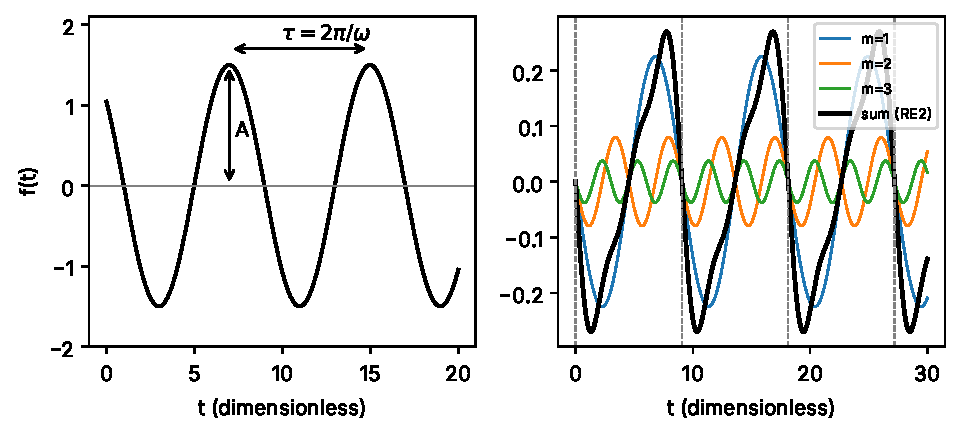
\includegraphics[width=0.95\linewidth]{figs/fourier-series_sinusoid.pdf}
\caption{Left: anatomy of a sinusoid $A\cos(\omega t+\varphi)$ with $A=1.5$, $\omega=2\pi/8$ and $\varphi=0.8$; the vertical arrow is the amplitude and the horizontal arrow one period $\tau=2\pi/\omega=8$ between successive maxima. Right: the three harmonics of the prime-2 wave RE2, \cref{eq:fourier-series-RE2}, and their sum (black), which repeats every $2\pi/\log2\approx9.065$ in $t$ (dashed lines). Both axes are dimensionless.}
\label{fig:fourier-series-sinusoid}
\end{figure}

\begin{checkpoint}
If you double the angular frequency of a sinusoid, what happens to its period? What happens to its amplitude?
\end{checkpoint}
\checkanswer{The period $2\pi/\omega$ halves. The amplitude is unchanged: $A$ and $\omega$ are independent constants.}

\begin{keyideas}
\item A sinusoid $A\cos(\omega t+\varphi)$ has amplitude $A$, angular frequency $\omega$, phase constant $\varphi$ and period $\tau=2\pi/\omega$.
\item Equivalently $a\cos\omega t+b\sin\omega t$ with $A=\sqrt{a^2+b^2}$; or $\Re[Ze^{i\omega t}]$ with complex amplitude $Z=Ae^{i\varphi}=a-ib$.
\item Sinusoids with frequencies $\omega,2\omega,3\omega,\dots$ are harmonics; their sum repeats with the fundamental period $2\pi/\omega$. RE2 is such a sum, with period $2\pi/\log2=9.065$.
\end{keyideas}

%=====================================================================
\section{Superposition and beats}\label{sec:fourier-series-beats}
% DYK-BEGIN
\begin{didyouknow}{Tuning by Ear}
Play tones of 440 Hz and 442 Hz together and you hear a single pitch that swells and fades twice per second. The beat frequency is the difference of the two frequencies, here 2 Hz. Piano tuners and guitarists exploit this, adjusting a string until the beats slow down and vanish. Superposition turns a tiny frequency mismatch into something your ear detects easily.
\end{didyouknow}
% DYK-END

On a stretched string, two small waves add: the displacement is the sum of the separate displacements. This \textbf{superposition principle} holds whenever the governing equation is linear, and it is why sums of sinusoids are everywhere.

\subsection{Same frequency: still a sinusoid}

Adding two sinusoids of the same $\omega$ gives another sinusoid of that $\omega$. Using \cref{eq:fourier-series-phasor},
\begin{equation}
\Re[Z_1e^{i\omega t}]+\Re[Z_2e^{i\omega t}]=\Re[(Z_1+Z_2)e^{i\omega t}],
\end{equation}
because the real part of a sum is the sum of the real parts. So the complex amplitudes simply add like vectors in the plane. Sample Problem ``Amplitude and phase'' was an instance: $3\cos\omega t$ has $Z_1=3$, $4\sin\omega t$ has $Z_2=-4i$, and $|Z_1+Z_2|=|3-4i|=5$.

\subsection{Different frequencies: beats}

Now add two sinusoids of equal amplitude and different angular frequencies $\omega_1<\omega_2$. We need the sum-to-product identity. Start from the addition formulas
\begin{align}
\sin(u+v)&=\sin u\cos v+\cos u\sin v,\\
\sin(u-v)&=\sin u\cos v-\cos u\sin v .
\end{align}
Adding them,
\begin{equation}
\sin(u+v)+\sin(u-v)=2\sin u\cos v .
\end{equation}
Set $u+v=\alpha$ and $u-v=\beta$, that is $u=(\alpha+\beta)/2$ and $v=(\alpha-\beta)/2$:
\begin{equation}
\sin\alpha+\sin\beta=2\sin\frac{\alpha+\beta}{2}\cos\frac{\alpha-\beta}{2}.
\label{eq:fourier-series-sumprod}
\end{equation}
With $\alpha=\omega_2t$, $\beta=\omega_1t$, and writing $\bar\omega=(\omega_1+\omega_2)/2$ and $\Delta\omega=\omega_2-\omega_1$,
\begin{equation}
\sin\omega_1t+\sin\omega_2t=\underbrace{2\cos\!\left(\frac{\Delta\omega}{2}t\right)}_{\text{slow envelope}}\;\underbrace{\sin(\bar\omega t)}_{\text{fast carrier}} .
\label{eq:fourier-series-beats}
\end{equation}
When $\Delta\omega\ll\bar\omega$, the result looks like a fast oscillation at the average frequency $\bar\omega$ whose amplitude $2|\cos(\Delta\omega\, t/2)|$ swells and fades slowly. For these equal amplitudes the loudness envelope $|\cos(\Delta\omega\, t/2)|$ vanishes when $\Delta\omega\, t/2=\pi/2+j\pi$ for integer $j$, so successive silences are separated by
\begin{equation}
\tau_{\rm beat}=\frac{2\pi}{\Delta\omega}.
\label{eq:fourier-series-beatperiod}
\end{equation}
Complete silences need equal amplitudes. With amplitudes $A_1\neq A_2$, add the two complex amplitudes as in the previous subsection: their relative angle $\Delta\omega\,t$ turns steadily, so the length of their sum swings between $|A_1-A_2|$ and $A_1+A_2$ and never reaches zero. The beat period is still $2\pi/\Delta\omega$. In terms of ordinary frequency this is the familiar first-year result: the beat frequency is the difference $f_2-f_1$. Two tuning forks at 440~Hz and 442~Hz beat twice per second.

\begin{pitfall}
The envelope function $\cos(\Delta\omega\, t/2)$ itself has period $4\pi/\Delta\omega$, twice $\tau_{\rm beat}$. The beat period is half that because the ear (and any amplitude measurement) responds to $|\cos|$, which repeats twice as often as $\cos$.
\end{pitfall}

\begin{sample}{Beats between the primes 11 and 13}
Paper Eq.~(4) contains the terms $\sin(t\log 11)$ and $\sin(t\log 13)$ (with different amplitudes, but take them equal here). Find the carrier frequency, the carrier period, the beat period, and the number of carrier cycles per beat.

\textbf{Step 1: frequencies.} $\omega_1=\log11=2.397895$, $\omega_2=\log13=2.564949$.

\textbf{Step 2: average and difference.} $\bar\omega=(\log 11+\log 13)/2=\tfrac12\log 143=2.481422$. $\Delta\omega=\log13-\log11=\log(13/11)=0.167054$.

\textbf{Step 3: carrier period.} $2\pi/\bar\omega=2.5321$.

\textbf{Step 4: beat period.} From \cref{eq:fourier-series-beatperiod}, $\tau_{\rm beat}=2\pi/0.167054=37.61$.

\textbf{Step 5: cycles per beat.} $\tau_{\rm beat}/(2\pi/\bar\omega)=\bar\omega/\Delta\omega=14.85$.
\[
\boxed{\bar\omega=2.4814,\quad \tau_{\rm beat}=37.61,\quad \text{about 14.85 carrier cycles per beat}}
\]
\end{sample}

\begin{figure}[htbp]\centering
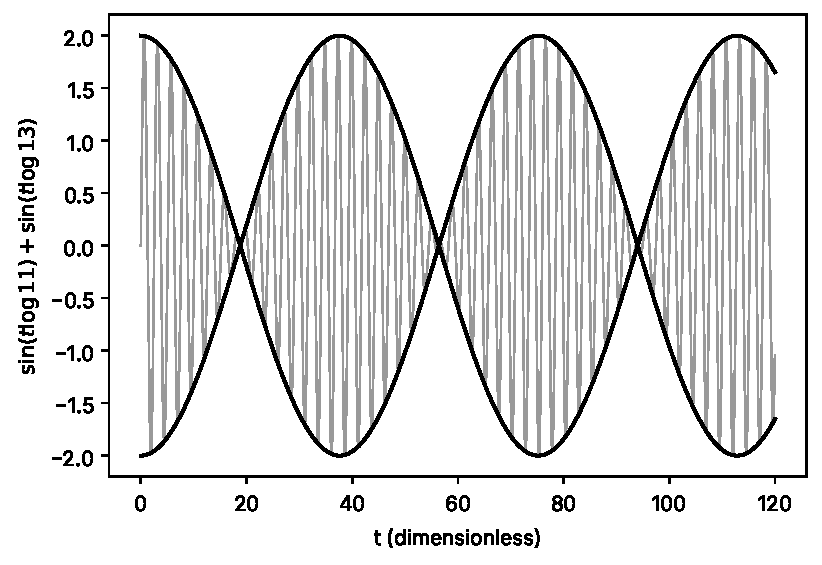
\includegraphics[width=0.85\linewidth]{figs/fourier-series_beats.pdf}
\caption{Beats: $\sin(t\log11)+\sin(t\log13)$ (gray) and its envelope $\pm2|\cos(t\log(13/11)/2)|$ (black). Silences recur every $\tau_{\rm beat}=2\pi/\log(13/11)\approx37.6$ in $t$. Both axes are dimensionless.}
\label{fig:fourier-series-beats}
\end{figure}

\begin{checkpoint}
In the sample problem above, how many silences (zeros of the envelope) occur for $0<t<100$?
\end{checkpoint}
\checkanswer{Silences occur at $t=(2j+1)\pi/\Delta\omega=(2j+1)\times18.81$, that is at $t\approx18.8$, $56.4$, $94.0$; the next is at $131.6$. So three.}

\begin{keyideas}
\item Superposition: for linear systems, oscillations add.
\item Same frequency: complex amplitudes add; the sum is one sinusoid.
\item Two equal-amplitude sinusoids with close frequencies produce beats, \cref{eq:fourier-series-beats}, with beat period $2\pi/\Delta\omega$.
\end{keyideas}

%=====================================================================
\section{Orthogonality of sines and cosines}\label{sec:fourier-series-orthogonality}

In 3D you find the $x$ component of a vector $\vec v$ by taking a dot product with the unit vector: $v_x=\vec v\cdot\hat x$. This works because $\hat x,\hat y,\hat z$ are \emph{orthogonal}: $\hat x\cdot\hat y=0$, and so on. Remarkably, sines and cosines of different whole-number frequencies behave in exactly this way, provided we replace the dot product by an integral of the product over one period. Chapter~\ref{ch:linear-algebra} develops this ``functions as vectors'' picture in general; here we only need the integrals.

\subsection{Product-to-sum identities}

From the addition formulas,
\begin{align}
\cos(\alpha-\beta)+\cos(\alpha+\beta)&=(\cos\alpha\cos\beta+\sin\alpha\sin\beta)+(\cos\alpha\cos\beta-\sin\alpha\sin\beta)=2\cos\alpha\cos\beta,\\
\cos(\alpha-\beta)-\cos(\alpha+\beta)&=2\sin\alpha\sin\beta,\\
\sin(\alpha+\beta)+\sin(\alpha-\beta)&=2\sin\alpha\cos\beta .
\end{align}
Hence
\begin{align}
\cos\alpha\cos\beta&=\tfrac12[\cos(\alpha-\beta)+\cos(\alpha+\beta)],\label{eq:fourier-series-pc}\\
\sin\alpha\sin\beta&=\tfrac12[\cos(\alpha-\beta)-\cos(\alpha+\beta)],\label{eq:fourier-series-ps}\\
\sin\alpha\cos\beta&=\tfrac12[\sin(\alpha+\beta)+\sin(\alpha-\beta)].\label{eq:fourier-series-psc}
\end{align}

\subsection{Two basic integrals}

Fix a half-width $L>0$ and integrate over the symmetric interval $[-L,L]$, which has length $2L$. For an integer $n$, define
\begin{equation}
I_c(n)=\int_{-L}^{L}\cos\frac{n\pi x}{L}\,\dd x,\qquad I_s(n)=\int_{-L}^{L}\sin\frac{n\pi x}{L}\,\dd x .
\end{equation}
For $n=0$ the cosine is $1$ and $I_c(0)=2L$. For $n\ne0$, an antiderivative of $\cos(n\pi x/L)$ is $(L/n\pi)\sin(n\pi x/L)$, so
\begin{equation}
I_c(n)=\frac{L}{n\pi}\left[\sin(n\pi)-\sin(-n\pi)\right]=\frac{2L}{n\pi}\sin(n\pi)=0,
\end{equation}
because $\sin(n\pi)=0$ for every integer $n$. Similarly, for $n\neq0$, an antiderivative of $\sin(n\pi x/L)$ is $-(L/n\pi)\cos(n\pi x/L)$, so
\begin{equation}
I_s(n)=-\frac{L}{n\pi}\left[\cos(n\pi)-\cos(-n\pi)\right]=0,
\end{equation}
because cosine is even, $\cos(-n\pi)=\cos(n\pi)$. For $n=0$, $I_s(0)=\int 0\,\dd x=0$. Summary: $I_s(n)=0$ always, and $I_c(n)=2L$ if $n=0$, otherwise $0$.

\subsection{The orthogonality relations}

Let $j,k$ be non-negative integers. Using \cref{eq:fourier-series-pc} with $\alpha=j\pi x/L$, $\beta=k\pi x/L$,
\begin{equation}
\int_{-L}^{L}\cos\frac{j\pi x}{L}\cos\frac{k\pi x}{L}\,\dd x=\tfrac12\left[I_c(j-k)+I_c(j+k)\right].
\end{equation}
Three cases:
\begin{itemize}
\item $j\ne k$: then $j-k\neq0$ and $j+k\ge1$, so both terms vanish: the integral is $0$.
\item $j=k\ge1$: $I_c(0)=2L$ and $I_c(2k)=0$, so the integral is $\tfrac12(2L)=L$.
\item $j=k=0$: both terms are $I_c(0)=2L$, so the integral is $2L$.
\end{itemize}
In the same way \cref{eq:fourier-series-ps,eq:fourier-series-psc} give the sine-sine and sine-cosine integrals. Introducing the \textbf{Kronecker delta} $\delta_{jk}$, equal to $1$ if $j=k$ and $0$ otherwise, the results are collected in \cref{tab:fourier-series-orth}.

\begin{table}[htbp]\centering
\caption{Orthogonality relations on $[-L,L]$ for non-negative integers $j,k$.}
\label{tab:fourier-series-orth}
\begin{tabular}{ll}
\toprule
integral over $[-L,L]$ & value\\
\midrule
$\int\cos\frac{j\pi x}{L}\cos\frac{k\pi x}{L}\,\dd x$ & $L\,\delta_{jk}$ for $j,k\ge1$; \quad $2L$ for $j=k=0$\\
$\int\sin\frac{j\pi x}{L}\sin\frac{k\pi x}{L}\,\dd x$ & $L\,\delta_{jk}$ for $j,k\ge1$\\
$\int\sin\frac{j\pi x}{L}\cos\frac{k\pi x}{L}\,\dd x$ & $0$ for all $j,k$\\
\bottomrule
\end{tabular}
\end{table}

For the sine-sine row with $j,k\ge1$: \cref{eq:fourier-series-ps} gives $\tfrac12[I_c(j-k)-I_c(j+k)]$, which is $0$ for $j\neq k$ and $\tfrac12(2L-0)=L$ for $j=k$. For the sine-cosine row, \cref{eq:fourier-series-psc} gives $\tfrac12[I_s(j+k)+I_s(j-k)]=0$.

Dividing the $j=k\ge1$ case by the interval length $2L$ gives a fact worth remembering: the \textbf{average of $\cos^2$ or $\sin^2$ over a whole number of periods is $\tfrac12$}.

\begin{sample}{Orthogonality on the paper's box}
Take $L=44.883$, the half-width of the paper's scale-1 box (RE3). Evaluate (a) $\int_{-L}^{L}\cos(2\pi x/L)\cos(3\pi x/L)\,\dd x$, (b) $\int_{-L}^{L}\cos^2(2\pi x/L)\,\dd x$, (c) $\int_{-L}^{L}1\cdot1\,\dd x$.

\textbf{Step 1 (a).} $j=2\neq k=3$, so by \cref{tab:fourier-series-orth} the integral is $0$. Directly: $\tfrac12[I_c(-1)+I_c(5)]=\tfrac12[0+0]=0$.

\textbf{Step 2 (b).} $j=k=2\ge1$: the integral is $L=44.883$.

\textbf{Step 3 (c).} $j=k=0$: the integral is $2L=89.766$.
\[
\boxed{0,\qquad 44.883,\qquad 89.766}
\]
A numerical quadrature (CHECKS) confirms all three.
\end{sample}

\begin{checkpoint}
Without computing anything, what is $\int_{-L}^{L}\sin(3\pi x/L)\cos(3\pi x/L)\,\dd x$?
\end{checkpoint}
\checkanswer{Zero: it is the sine-cosine row of \cref{tab:fourier-series-orth}. (Also $\sin\theta\cos\theta=\tfrac12\sin2\theta$, whose integral over whole periods vanishes.)}

\begin{keyideas}
\item On $[-L,L]$ the functions $1$, $\cos(k\pi x/L)$, $\sin(k\pi x/L)$ ($k=1,2,\dots$) are mutually orthogonal: the integral of the product of any two different ones is zero.
\item The ``squared length'' of $\cos(k\pi x/L)$ or $\sin(k\pi x/L)$ is $L$; that of the constant $1$ is $2L$.
\item The average of $\cos^2$ or $\sin^2$ over whole periods is $\tfrac12$.
\end{keyideas}

%=====================================================================
\section{Fourier series}\label{sec:fourier-series-series}

A guitar string of length $\ell$ fixed at both ends vibrates in standing-wave modes $\sin(k\pi x/\ell)$, $k=1,2,3,\dots$. Pluck it into some triangular shape and the subsequent motion is a superposition of these modes. Joseph Fourier's bold claim (1807) was that essentially any shape can be written as such a superposition. Orthogonality tells us how to find the recipe.

\subsection{Definition}

Let $f$ be periodic with period $2L$, so $f(x+2L)=f(x)$. Its \textbf{Fourier series} is
\begin{equation}
f(x)=\frac{a_0}{2}+\sum_{k=1}^{\infty}\left[a_k\cos\frac{k\pi x}{L}+b_k\sin\frac{k\pi x}{L}\right].
\label{eq:fourier-series-FS}
\end{equation}
Each term has period $2L/k$, which fits exactly $k$ times into $2L$. So each term repeats after $2L$, and the whole right-hand side has period $2L$, consistent with the left. A function defined only on $[-L,L]$ can always be treated as one period of its \textbf{periodic extension}, obtained by copying the graph on $[-L,L]$ into $[L,3L]$, $[3L,5L]$, and so on.

\subsection{Deriving the coefficients}

Suppose \cref{eq:fourier-series-FS} holds. Pick an integer $n\ge1$, multiply both sides by $\cos(n\pi x/L)$, and integrate over $[-L,L]$, integrating the right-hand side term by term (see the box below for when this is allowed):
\begin{align}
\int_{-L}^{L}f(x)\cos\frac{n\pi x}{L}\dd x
&=\frac{a_0}{2}\int_{-L}^{L}\cos\frac{n\pi x}{L}\dd x
+\sum_{k\ge1}a_k\int_{-L}^{L}\cos\frac{k\pi x}{L}\cos\frac{n\pi x}{L}\dd x\nonumber\\
&\quad+\sum_{k\ge1}b_k\int_{-L}^{L}\sin\frac{k\pi x}{L}\cos\frac{n\pi x}{L}\dd x\\
&=\frac{a_0}{2}\cdot0+\sum_{k\ge1}a_k\,L\,\delta_{kn}+\sum_{k\ge1}b_k\cdot 0\quad\text{(\cref{tab:fourier-series-orth})}\\
&=a_n L .
\end{align}
Every term except one is killed by orthogonality. So
\begin{equation}
a_n=\frac1L\int_{-L}^{L}f(x)\cos\frac{n\pi x}{L}\,\dd x .
\label{eq:fourier-series-an}
\end{equation}
For $n=0$, integrate \cref{eq:fourier-series-FS} directly (multiply by $\cos 0=1$): the constant term gives $(a_0/2)(2L)=a_0L$ and every other term integrates to zero, so $a_0=(1/L)\int f\,\dd x$. This is \cref{eq:fourier-series-an} with $n=0$; that is the reason for writing the constant term as $a_0/2$. Multiplying instead by $\sin(n\pi x/L)$ and using the sine rows of \cref{tab:fourier-series-orth},
\begin{equation}
b_n=\frac1L\int_{-L}^{L}f(x)\sin\frac{n\pi x}{L}\,\dd x .
\label{eq:fourier-series-bn}
\end{equation}
Note that $a_0/2=(1/2L)\int f\,\dd x$ is the \textbf{average value} of $f$ over a period.

\begin{beyond}
\textbf{What we take on trust: convergence.} The derivation assumed that the series converges to $f$ and may be integrated term by term. The standard theorem (Dirichlet's theorem) states: if $f$ has period $2L$ and, on one period, $f$ and $f'$ are continuous except for finitely many jump discontinuities, then the Fourier series converges at every $x$; its sum is $f(x)$ wherever $f$ is continuous and is the midpoint $\tfrac12[f(x^-)+f(x^+)]$ at a jump. For such $f$ the coefficient formulas \cref{eq:fourier-series-an,eq:fourier-series-bn} are valid. Riley, Hobson and Bence~\cite{rhb} state these (Dirichlet) conditions in their chapter on Fourier series but do not prove the theorem; a proof, via the so-called Dirichlet kernel, is found in texts on Fourier analysis or real analysis. Every function expanded in a Fourier series in this chapter satisfies these conditions.
\end{beyond}

\begin{sample}{The square wave}
Find the Fourier series of the square wave of period $2\pi$: $f(x)=-1$ for $-\pi<x<0$ and $f(x)=+1$ for $0<x<\pi$.

\textbf{Step 1: set $L=\pi$.} Then $k\pi x/L=kx$.

\textbf{Step 2: cosine coefficients.} $a_n=\frac1\pi\int_{-\pi}^{\pi}f(x)\cos nx\,\dd x$. Split at $0$ and substitute $x\to-x$ in the left half:
$\int_{-\pi}^0(-1)\cos nx\,\dd x=-\int_0^{\pi}\cos nx\,\dd x$, which cancels the right half $\int_0^\pi\cos nx\,\dd x$. So $a_n=0$ for all $n$ (including $n=0$: the average is zero).

\textbf{Step 3: sine coefficients.} The same substitution gives $\int_{-\pi}^0(-1)\sin nx\,\dd x=\int_0^\pi\sin nx\,\dd x$ (two sign changes), so
\[
b_n=\frac2\pi\int_0^\pi\sin nx\,\dd x=\frac2\pi\left[-\frac{\cos nx}{n}\right]_0^\pi=\frac{2}{n\pi}\left(1-\cos n\pi\right)=\frac{2}{n\pi}\left(1-(-1)^n\right).
\]
So $b_n=4/(n\pi)$ for odd $n$ and $0$ for even $n$.

\textbf{Step 4: the series.}
\[
\boxed{f(x)=\frac4\pi\left(\sin x+\frac{\sin3x}{3}+\frac{\sin5x}{5}+\cdots\right)}
\]
The first coefficient is $b_1=4/\pi=1.2732$: the best-fitting single sine (best in the mean-square sense, as shown in \cref{sec:fourier-series-parseval}) is \emph{taller} than the square wave.

\textbf{Step 5: a bonus.} At $x=\pi/2$, $f=1$ and $\sin(n\pi/2)=1,-1,1,\dots$ for $n=1,3,5,\dots$, so $1=\frac4\pi(1-\frac13+\frac15-\cdots)$, Leibniz's series $\pi/4=1-\tfrac13+\tfrac15-\cdots$. At the jump $x=0$ every term vanishes, giving $0$, the midpoint of $-1$ and $+1$, as Dirichlet's theorem promises.
\end{sample}

\begin{pycode}
import numpy as np
from scipy.integrate import quad

# Fourier sine coefficients of the square wave, by numerical integration
def f(x):
    return np.sign(x)            # -1 on (-pi,0), +1 on (0,pi)

for n in range(1, 6):
    bn = quad(lambda x: f(x)*np.sin(n*x), -np.pi, np.pi, points=[0])[0]/np.pi
    exact = 4/(n*np.pi) if n % 2 == 1 else 0.0
    print(n, round(bn, 6), round(exact, 6))
\end{pycode}

\subsection{The Gibbs phenomenon}\label{sec:fourier-series-gibbs}

Truncate the square-wave series after $K$ nonzero terms:
\begin{equation}
S_K(x)=\frac4\pi\sum_{j=1}^{K}\frac{\sin((2j-1)x)}{2j-1}.
\end{equation}
\Cref{fig:fourier-series-gibbs} shows that near the jump $S_K$ overshoots the value $1$, and the overshoot does not shrink to zero as $K$ grows; it settles to a fixed size and only gets narrower. This is the \textbf{Gibbs phenomenon}. We can compute the size of the overshoot exactly.

\textbf{Locating the first peak.} Differentiate term by term (a finite sum, so this is allowed):
\begin{equation}
S_K'(x)=\frac4\pi\sum_{j=1}^K\cos((2j-1)x)=\frac4\pi\,\Re\sum_{j=1}^K e^{i(2j-1)x}.
\end{equation}
The sum is geometric (Chapter~\ref{ch:series}) with first term $e^{ix}$ and ratio $e^{2ix}$:
\begin{equation}
\sum_{j=1}^K e^{i(2j-1)x}=e^{ix}\,\frac{1-e^{2iKx}}{1-e^{2ix}} .
\end{equation}
Divide numerator and denominator of $e^{ix}/(1-e^{2ix})$ by $e^{ix}$: it equals $1/(e^{-ix}-e^{ix})=1/(-2i\sin x)=i/(2\sin x)$, using $e^{ix}-e^{-ix}=2i\sin x$ and $1/(-i)=i$. Therefore
\begin{equation}
\sum_{j=1}^K e^{i(2j-1)x}=\frac{i\,(1-\cos2Kx-i\sin 2Kx)}{2\sin x}=\frac{\sin2Kx+i(1-\cos2Kx)}{2\sin x},
\end{equation}
whose real part is $\sin(2Kx)/(2\sin x)$. Hence, for $0<x<\pi$,
\begin{equation}
S_K'(x)=\frac{2}{\pi}\,\frac{\sin 2Kx}{\sin x}.
\end{equation}
This is positive for $0<x<\pi/(2K)$ (there $\sin 2Kx>0$ and $\sin x>0$) and changes sign at $x^*=\pi/(2K)$. So $S_K$ rises from $0$ at $x=0$ to a local maximum at $x^*$. This is the \emph{first} peak to the right of the jump, and it is the one whose height we compute. \Cref{fig:fourier-series-gibbs} shows that it is also the tallest, the later peaks (at the other sign changes of $\sin 2Kx$) being lower. We do not prove that last statement, and nothing below depends on it.

\textbf{Height of the peak.} At $x^*$, the $j$-th term has argument $u_j=(2j-1)\pi/(2K)$. Since $1/(2j-1)=(\pi/2K)/u_j$,
\begin{equation}
S_K(x^*)=\frac4\pi\cdot\frac{\pi}{2K}\sum_{j=1}^K\frac{\sin u_j}{u_j}=\frac2\pi\sum_{j=1}^K\frac{\sin u_j}{u_j}\,\Delta u,\qquad \Delta u=\frac\pi K .
\end{equation}
The points $u_j$ are the midpoints of $K$ equal subintervals of $[0,\pi]$ (subinterval $j$ is $[(j-1)\pi/K,\,j\pi/K]$, whose midpoint is $(j-\tfrac12)\pi/K=u_j$). So the sum is a Riemann sum (the midpoint rule) for an integral over $[0,\pi]$. The integrand $\sin u/u$ is continuous on $[0,\pi]$ once we give it its limiting value $1$ at $u=0$, and for a continuous function the sum of (value at one point of each subinterval) $\times$ (subinterval width) tends to the integral as the widths tend to zero; that is the definition of the definite integral. Hence, as $K\to\infty$,
\begin{equation}
S_K(x^*)\to\frac2\pi\int_0^\pi\frac{\sin u}{u}\,\dd u=\frac2\pi\,\mathrm{Si}(\pi)=1.17898,
\label{eq:fourier-series-gibbs}
\end{equation}
where $\mathrm{Si}(z)=\int_0^z(\sin u/u)\,\dd u$ is the \emph{sine integral}, a tabulated function with $\mathrm{Si}(\pi)=1.851937$ (computed in CHECKS with \texttt{scipy.special.sici}). In the limit $K\to\infty$ the overshoot above $1$ is $0.17898$, which is $8.95\%$ of the total jump $2$, about $9\%$. For finite $K$ the first peak is higher (for $K=1$ it is $4/\pi=1.273$, an overshoot of $13.7\%$ of the jump), so the overshoot approaches about $9\%$ but never decays to zero, however many terms you keep. For $K=50$, the finite sum gives $S_{50}(x^*)=1.1790$.

\begin{figure}[htbp]\centering
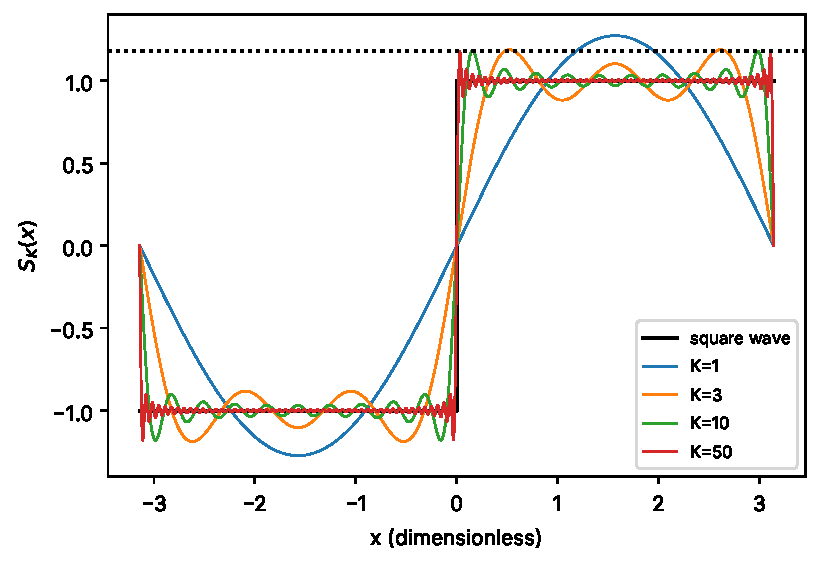
\includegraphics[width=0.85\linewidth]{figs/fourier-series_gibbs.pdf}
\caption{Partial sums $S_K$ of the square-wave series with $K=1,3,10,50$ terms. The overshoot near the jump at $x=0$ tends to $(2/\pi)\mathrm{Si}(\pi)=1.179$ (dotted line), about $9\%$ of the jump, and moves closer to the jump as $K$ grows. Axes dimensionless.}
\label{fig:fourier-series-gibbs}
\end{figure}

\begin{pitfall}
Adding more terms does \emph{not} remove the Gibbs overshoot. It squeezes it into a narrower region (width $\propto1/K$), so the series still converges at each fixed $x\neq0$, but the overshoot at the first peak next to the jump approaches about $9\%$ of the jump instead of zero. Jumps are expensive for Fourier series; we will see that the paper's cosine basis avoids jumps at the walls for even functions.
\end{pitfall}

\begin{keyideas}
\item A $2L$-periodic function has the Fourier series \cref{eq:fourier-series-FS} with $a_n=\frac1L\int f\cos\frac{n\pi x}{L}$, $b_n=\frac1L\int f\sin\frac{n\pi x}{L}$, derived by orthogonality.
\item The series converges to $f$ where $f$ is continuous and to the midpoint at jumps (Dirichlet's theorem, taken on trust).
\item Near a jump, the overshoot of the partial sums tends to about $9\%$ of the jump as $K\to\infty$ and never decays to zero (Gibbs phenomenon), \cref{eq:fourier-series-gibbs}.
\end{keyideas}

%=====================================================================
\section{The complex form}\label{sec:fourier-series-complex}

Sines and cosines come in pairs; complex exponentials package each pair into one function and make the algebra shorter. They will be the natural language of the Fourier transform in Chapter~\ref{ch:fourier-transform}.

\subsection{Orthogonality of complex exponentials}

For integers $k$ and $l$ consider $\int_{-L}^{L}e^{ik\pi x/L}\,\overline{e^{il\pi x/L}}\,\dd x$, where the overbar is the complex conjugate (Chapter~\ref{ch:complex}); for complex functions the ``dot product'' conjugates the second factor. The reason for the conjugate: with it, the product of a function with itself is $\int f\bar f\,\dd x=\int|f|^2\dd x\ge0$, a genuine squared length; without it, $\int_{-L}^{L}e^{i\pi x/L}e^{i\pi x/L}\dd x$ would be $0$ (by the computation below with $k-l$ replaced by $2$) even though the function is never zero. To integrate a complex-valued function of the real variable $x$, integrate its real and imaginary parts separately: $\int(u+iv)\,\dd x=\int u\,\dd x+i\int v\,\dd x$. For a real constant $\alpha\neq0$ this gives
\[
\int e^{i\alpha x}\dd x=\int\cos\alpha x\,\dd x+i\int\sin\alpha x\,\dd x=\frac{\sin\alpha x}{\alpha}-i\frac{\cos\alpha x}{\alpha}=\frac{e^{i\alpha x}}{i\alpha},
\]
where the last step multiplies $\cos\alpha x+i\sin\alpha x$ by $1/i=-i$. So complex exponentials integrate exactly like real ones. Since $\overline{e^{i\theta}}=e^{-i\theta}$, the integrand is $e^{i(k-l)\pi x/L}$. If $k=l$ it is $1$ and the integral is $2L$. If $k\neq l$,
\begin{equation}
\int_{-L}^{L}e^{i(k-l)\pi x/L}\,\dd x=\frac{L}{i(k-l)\pi}\left[e^{i(k-l)\pi}-e^{-i(k-l)\pi}\right]=\frac{L}{i(k-l)\pi}\,2i\sin((k-l)\pi)=0 .
\end{equation}
So
\begin{equation}
\int_{-L}^{L}e^{ik\pi x/L}e^{-il\pi x/L}\,\dd x=2L\,\delta_{kl}.
\label{eq:fourier-series-orthexp}
\end{equation}

\subsection{The complex Fourier series}

The complex Fourier series of a $2L$-periodic function is
\begin{equation}
f(x)=\sum_{k=-\infty}^{\infty}\hat f_k\,e^{ik\pi x/L},\qquad
\hat f_k=\frac1{2L}\int_{-L}^{L}f(x)\,e^{-ik\pi x/L}\,\dd x .
\label{eq:fourier-series-complexFS}
\end{equation}
The coefficient formula follows exactly as before: multiply the series by $e^{-in\pi x/L}$, integrate over $[-L,L]$ term by term, and use \cref{eq:fourier-series-orthexp}; only $k=n$ survives, giving $2L\hat f_n$. Notice the sum runs over \emph{negative} $k$ too.

\paragraph{Relation to the real form.} Substitute $\cos\theta=(e^{i\theta}+e^{-i\theta})/2$ and $\sin\theta=(e^{i\theta}-e^{-i\theta})/(2i)$ into one term of \cref{eq:fourier-series-FS}, with $\theta=k\pi x/L$:
\begin{align}
a_k\cos\theta+b_k\sin\theta&=\frac{a_k}{2}(e^{i\theta}+e^{-i\theta})+\frac{b_k}{2i}(e^{i\theta}-e^{-i\theta})\\
&=\frac{a_k-ib_k}{2}e^{i\theta}+\frac{a_k+ib_k}{2}e^{-i\theta}\quad\text{(using $1/i=-i$)}.
\end{align}
Comparing with \cref{eq:fourier-series-complexFS},
\begin{equation}
\hat f_0=\frac{a_0}{2},\qquad \hat f_k=\frac{a_k-ib_k}{2},\qquad \hat f_{-k}=\frac{a_k+ib_k}{2}\qquad(k\ge1).
\label{eq:fourier-series-realcomplex}
\end{equation}
For a real function, $a_k$ and $b_k$ are real, so $\hat f_{-k}=\overline{\hat f_k}$. You can also see this directly: conjugating the integral in \cref{eq:fourier-series-complexFS} with $f$ real flips the sign of the exponent and turns $\hat f_k$ into $\hat f_{-k}$.

\begin{sample}{RE2 in complex form}
Write the prime-2 wave \cref{eq:fourier-series-RE2} as a complex Fourier series.

\textbf{Step 1: choose the period.} RE2 has period $2\pi/\log2$, so set $2L=2\pi/\log 2$. Then $k\pi/L=k\log2$, and term $m$ of RE2 is harmonic $k=m$.

\textbf{Step 2: read off real coefficients.} Term $m$ is $-A_m\sin(m t\log2)$, so $a_m=0$ and $b_m=-A_m$ for $m=1,2,3$; all other coefficients vanish.

\textbf{Step 3: apply \cref{eq:fourier-series-realcomplex}.} $\hat f_m=(0-i(-A_m))/2=iA_m/2$ and $\hat f_{-m}=-iA_m/2$.

\textbf{Step 4: numbers.} Using $A_m$ from the earlier sample problem:
\[
\boxed{\hat f_{\pm1}=\pm0.1125\,i,\quad \hat f_{\pm2}=\pm0.0398\,i,\quad \hat f_{\pm3}=\pm0.0188\,i}
\]
and all other $\hat f_k=0$. Six nonzero complex coefficients describe the whole wave for all $t$. Check: $\hat f_{-m}=\overline{\hat f_m}$, as it must be for a real function.
\end{sample}

\begin{keyideas}
\item $f(x)=\sum_k\hat f_ke^{ik\pi x/L}$ with $\hat f_k=\frac1{2L}\int f e^{-ik\pi x/L}\dd x$, by the orthogonality \cref{eq:fourier-series-orthexp}.
\item $\hat f_k=(a_k-ib_k)/2$; for real $f$, $\hat f_{-k}=\overline{\hat f_k}$.
\end{keyideas}

%=====================================================================
\section{Parseval's theorem and best approximation}\label{sec:fourier-series-parseval}

\subsection{Parseval's theorem}

How ``big'' is a function? A natural measure, the one behind every rms in the paper, is its \textbf{mean square} over a period, $\langle|f|^2\rangle=\frac1{2L}\int_{-L}^{L}|f|^2\,\dd x$ (for real $f$, $|f|^2=f^2$ and we write simply $\langle f^2\rangle$), and its square root, the root mean square (rms). Parseval's theorem says the mean square is the sum of the squared moduli of the Fourier coefficients, exactly as the squared length of a 3D vector is $v_x^2+v_y^2+v_z^2$.

\textbf{Derivation.} Write $|f|^2=f\,\bar f$ and insert the complex series for $f$ and for $\bar f$ (for $\bar f$, conjugate each term, and use a second summation index $l$):
\begin{align}
\frac1{2L}\int_{-L}^{L}|f|^2\dd x
&=\frac1{2L}\int_{-L}^{L}\Big(\sum_k\hat f_ke^{ik\pi x/L}\Big)\Big(\sum_l\overline{\hat f_l}\,e^{-il\pi x/L}\Big)\dd x\\
&=\sum_k\sum_l\hat f_k\overline{\hat f_l}\;\frac1{2L}\int_{-L}^{L}e^{i(k-l)\pi x/L}\dd x\\
&=\sum_k\sum_l\hat f_k\overline{\hat f_l}\;\delta_{kl}\qquad\text{(\cref{eq:fourier-series-orthexp})}\\
&=\sum_k|\hat f_k|^2 .
\label{eq:fourier-series-parseval}
\end{align}
In real form, \cref{eq:fourier-series-realcomplex} gives $|\hat f_0|^2=a_0^2/4$ and $|\hat f_k|^2=|\hat f_{-k}|^2=(a_k^2+b_k^2)/4$, so the pair $\pm k$ contributes $(a_k^2+b_k^2)/2$:
\begin{equation}
\frac1{2L}\int_{-L}^{L}f^2\,\dd x=\frac{a_0^2}{4}+\frac12\sum_{k=1}^{\infty}\left(a_k^2+b_k^2\right).
\label{eq:fourier-series-parsevalreal}
\end{equation}

\begin{beyond}
The interchange of the double sum with the integral needs justification. Parseval's theorem holds for every $f$ with $\int_{-L}^{L}|f|^2\dd x$ finite, including functions with jumps such as the square wave; Riley, Hobson and Bence~\cite{rhb} give the formal term-by-term derivation shown above; the rigorous proof rests on the completeness of the trigonometric system (mean-square convergence of Fourier series) and is found in texts on Fourier analysis.
\end{beyond}

A single sinusoid $A\cos(\omega t+\varphi)$ has $a^2+b^2=A^2$, so its mean square is $A^2/2$ and its rms is $A/\sqrt2$, the familiar rms of an AC voltage. Parseval says that for a sum of harmonics, the mean squares simply add: there are no cross terms, because of orthogonality.

\begin{sample}{Parseval for the square wave}
Use Parseval on the square wave to evaluate $\sum_{\text{odd }k}1/k^2$.

\textbf{Step 1: left side.} $f^2=1$ everywhere (except at isolated points, which do not affect integrals), so the mean square is $1$.

\textbf{Step 2: right side.} $a_k=0$, $b_k=4/(k\pi)$ for odd $k$: $\frac12\sum_{\text{odd}}16/(k^2\pi^2)=\frac{8}{\pi^2}\sum_{\text{odd}}\frac1{k^2}$.

\textbf{Step 3: equate.}
\[
\boxed{1+\frac1{9}+\frac1{25}+\cdots=\frac{\pi^2}{8}=1.2337}
\]
\end{sample}

\begin{sample}{The rms of the prime-2 wave}
Find the rms of RE2 over a period.

\textbf{Step 1: Parseval in real form.} RE2 has $b_m=-A_m$, so the mean square is $\frac12\sum_{m=1}^3A_m^2$.

\textbf{Step 2: squares.} $A_m^2=1/(\pi^2m^22^m)$: $\sum_m 1/(m^22^m)=\frac12+\frac1{16}+\frac1{72}=0.576389$.

\textbf{Step 3: mean square.} $0.576389/(2\pi^2)=0.029200$.

\textbf{Step 4: rms.}
\[
\boxed{\text{rms of RE2}=\sqrt{0.029200}=0.1709}
\]
Most of it comes from $m=1$: $A_1/\sqrt2=0.1592$ on its own. We return to this number in the Paper connection.
\end{sample}

\subsection{Truncated Fourier series are the best approximations}

Suppose you may use only finitely many harmonics. Which coefficients should you use? We show that the Fourier coefficients themselves are the best choice in the mean-square sense. We do it for even functions and cosines (the case used in the paper); the general case is identical.

Let $f$ be even on $[-L,L]$ and write its cosine series in the convention the paper uses,
\begin{equation}
f(x)=\sum_{k=0}^{\infty}c_k\cos\frac{k\pi x}{L},\qquad c_0=\frac1{2L}\int_{-L}^{L}f\,\dd x,\quad c_k=\frac1L\int_{-L}^{L}f\cos\frac{k\pi x}{L}\dd x\ (k\ge1),
\label{eq:fourier-series-cosconv}
\end{equation}
so $c_0=a_0/2$ and $c_k=a_k$. Approximate $f$ by $g(x)=\sum_{k=0}^{M-1}d_k\cos(k\pi x/L)$ with arbitrary numbers $d_k$, and measure the error by $\mathcal{E}=\frac1{2L}\int_{-L}^{L}(f-g)^2\dd x$ (we write $\mathcal{E}$, not $E$, because this book reserves $E$ for energies). Expand the square:
\begin{equation}
\mathcal{E}=\frac1{2L}\int f^2\dd x-2\sum_{k<M}d_k\frac1{2L}\int f\cos\frac{k\pi x}{L}\dd x+\sum_{j,k<M}d_jd_k\frac1{2L}\int\cos\frac{j\pi x}{L}\cos\frac{k\pi x}{L}\dd x .
\end{equation}
By \cref{tab:fourier-series-orth}, the last average is $\nu_k\delta_{jk}$ with $\nu_0=1$ and $\nu_k=\tfrac12$ for $k\ge1$. By \cref{eq:fourier-series-cosconv}, the middle average is $\nu_kc_k$ (for $k\ge1$ it is $c_k/2$; for $k=0$ it is $c_0$). Hence
\begin{equation}
\mathcal{E}=\langle f^2\rangle+\sum_{k<M}\nu_k\left(d_k^2-2d_kc_k\right)
=\langle f^2\rangle+\sum_{k<M}\nu_k(d_k-c_k)^2-\sum_{k<M}\nu_kc_k^2,
\label{eq:fourier-series-best}
\end{equation}
where we completed the square, $d^2-2dc=(d-c)^2-c^2$. Only the middle sum depends on the $d_k$, and it is a sum of non-negative terms, smallest (zero) when $d_k=c_k$. So:
\begin{itemize}
\item the truncated Fourier series is the best mean-square approximation with $M$ cosines;
\item its error is $\mathcal{E}_{\min}=\langle f^2\rangle-\sum_{k<M}\nu_kc_k^2\ge0$ (Bessel's inequality), which tends to zero as $M\to\infty$ by Parseval.
\end{itemize}
This is a first example of \emph{least squares} (Chapter~\ref{ch:least-squares}): with an orthogonal basis, the least-squares coefficients are simply projections. The paper also determines cosine coefficients by least squares, but for a different target, the energy levels, so its $c_k$ are not the projections of any known function (Chapter~\ref{ch:fitting}).

\begin{checkpoint}
Does the rms of RE2 depend on where you start the period, or on the phases of the three terms?
\end{checkpoint}
\checkanswer{No. The mean over any full period is the same, and Parseval uses only $|\hat f_k|^2$, which ignores phases.}

\begin{keyideas}
\item Parseval: $\langle|f|^2\rangle=\sum_k|\hat f_k|^2=\frac{a_0^2}4+\frac12\sum(a_k^2+b_k^2)$; mean squares of orthogonal pieces add.
\item A sinusoid of amplitude $A$ has rms $A/\sqrt2$. RE2 has rms $0.1709$.
\item Truncated Fourier series minimize the mean-square error among all combinations of the same harmonics, \cref{eq:fourier-series-best}.
\end{keyideas}

%=====================================================================
\section{Even and odd functions; the cosine basis on \texorpdfstring{$[-L,L]$}{[-L,L]}}\label{sec:fourier-series-evenodd}
% DYK-BEGIN
\begin{didyouknow}{Fourier Faced Skeptics}
Joseph Fourier presented his theory of heat flow, built on expanding functions in sines and cosines, to the Paris Academy in 1807. Examiners, including Lagrange, doubted that arbitrary functions, even ones with corners or jumps, could be written as such series. Fourier won an Academy prize for the work a few years later, and his book \emph{Th\'eorie analytique de la chaleur} finally appeared in 1822.
\end{didyouknow}
% DYK-END

\subsection{Definitions and rules}

A function is \textbf{even} if $f(-x)=f(x)$ for all $x$ (mirror-symmetric about $x=0$: $\cos$, $x^2$, $|x|$) and \textbf{odd} if $f(-x)=-f(x)$ (antisymmetric: $\sin$, $x$, $x^3$). Most functions are neither, but every function splits uniquely into an even and an odd part:
\begin{equation}
f(x)=\underbrace{\frac{f(x)+f(-x)}{2}}_{f_{\rm e}(x)}+\underbrace{\frac{f(x)-f(-x)}{2}}_{f_{\rm o}(x)} .
\end{equation}
(Replace $x$ by $-x$ in $f_{\rm e}$: the two terms swap, so $f_{\rm e}$ is even; in $f_{\rm o}$ they swap and change sign, so $f_{\rm o}$ is odd. Uniqueness: if also $f=g_{\rm e}+g_{\rm o}$ with $g_{\rm e}$ even and $g_{\rm o}$ odd, then $f(-x)=g_{\rm e}(x)-g_{\rm o}(x)$, so $f(x)+f(-x)=2g_{\rm e}(x)$ and $f(x)-f(-x)=2g_{\rm o}(x)$, which says $g_{\rm e}=f_{\rm e}$ and $g_{\rm o}=f_{\rm o}$.)

Products obey sign rules like multiplying $\pm1$. If $f,g$ are even, $(fg)(-x)=f(x)g(x)$: even. If both are odd, $(fg)(-x)=(-f(x))(-g(x))=f(x)g(x)$: even. If $f$ is even and $g$ odd, $(fg)(-x)=f(x)(-g(x))$: odd.

\textbf{Integrals over symmetric intervals.} If $h$ is odd, split $\int_{-L}^{L}h=\int_{-L}^{0}h+\int_0^Lh$ and in the first piece substitute $x=-y$ ($\dd x=-\dd y$):
\begin{equation}
\int_{-L}^{0}h(x)\,\dd x=\int_{L}^{0}h(-y)(-\dd y)=\int_0^Lh(-y)\,\dd y=-\int_0^Lh(y)\,\dd y,
\end{equation}
so $\int_{-L}^{L}h\,\dd x=0$. If $h$ is even, the same substitution gives $+\int_0^Lh$, so $\int_{-L}^{L}h=2\int_0^Lh$.

\subsection{Cosine and sine series}

If $f$ is even, $f(x)\sin(k\pi x/L)$ is odd, so every $b_k=0$; and $f\cos(k\pi x/L)$ is even, so $a_k=\frac2L\int_0^Lf\cos(k\pi x/L)\dd x$. An even function has a \textbf{pure cosine series}. If $f$ is odd, all $a_k=0$ and it has a \textbf{pure sine series} (the square wave of \cref{sec:fourier-series-series} was odd, and indeed had only sines).

\subsection{The cosine basis on \texorpdfstring{$[-L,L]$}{[-L,L]}}

Why care about evenness? In Chapter~\ref{ch:bound-states} you will see that a potential symmetric under $x\to-x$ (as the Wu--Sprung potential is) has states of definite parity, and that a correction which keeps the symmetry must itself be even. So the natural expansion of an even correction on the box $[-L,L]$ is the \textbf{cosine basis}
\begin{equation}
\phi_k(x)=\cos\frac{k\pi x}{L},\qquad k=0,1,\dots,M-1,
\label{eq:fourier-series-basis}
\end{equation}
with coefficients given by \cref{eq:fourier-series-cosconv}. The basis function $\phi_k$ has wavelength $2L/k$ and wavenumber $k\pi/L$ (radians per unit $x$); $\phi_0=1$ is the constant.

\begin{pitfall}
Conventions for the constant term differ. In \cref{eq:fourier-series-FS} the constant is $a_0/2$ with $a_0=\frac1L\int f$. In the paper's form $\sum_kc_k\cos(k\pi x/L)$ the constant is $c_0$ itself, so $c_0=\frac1{2L}\int f$, the average. Mixing the two conventions doubles or halves the constant.
\end{pitfall}

\paragraph{No jumps at the walls.} The cosine series of $f$ on $[-L,L]$ represents the $2L$-periodic extension of $f$. Just to the right of $x=L$ the extension equals $f(-L+\varepsilon)$, which tends to $f(-L)$; just to the left it is $f(L)$. For an even function $f(-L)=f(L)$, so the extension has \emph{no jump} at the walls and there is no Gibbs overshoot there. There is generally a \emph{kink}: the slope just left of $L$ is $f'(L)$ and just right of it is $f'(-L)=-f'(L)$.

\paragraph{How fast do the coefficients fall?} Integrate by parts twice. With $q=k\pi/L$ and $k\ge1$,
\begin{align}
c_k&=\frac2L\int_0^Lf\cos qx\,\dd x=\frac2L\left[\frac{f\sin qx}{q}\right]_0^L-\frac{2}{Lq}\int_0^Lf'\sin qx\,\dd x\\
&=-\frac2{Lq}\left(\left[-\frac{f'\cos qx}{q}\right]_0^L+\frac1q\int_0^Lf''\cos qx\,\dd x\right)\quad\text{($\sin k\pi=\sin0=0$)}\\
&=\frac{2L}{k^2\pi^2}\Big[(-1)^kf'(L)-f'(0^+)\Big]-\frac{2L}{k^2\pi^2}\int_0^Lf''\cos qx\,\dd x,
\label{eq:fourier-series-decay}
\end{align}
using $\cos(k\pi)=(-1)^k$ and $2/(Lq^2)=2L/(k^2\pi^2)$. When $f$ is smooth, the remaining integral itself shrinks as $k$ grows (integrate by parts again), so a kink makes $c_k$ fall like $1/k^2$, while a jump would make coefficients fall only like $1/k$ (Problem~25). Smooth features need few cosines; sharp features need many.

\begin{sample}{The cosine series of $|x|$ on the paper's box}
Expand $f(x)=|x|$ on $[-L,L]$ with $L=44.883$, and find the rms error of keeping only $k=0,1,2,3$ ($M=4$).

\textbf{Step 1: constant.} $c_0=\frac1{2L}\int_{-L}^{L}|x|\dd x=\frac1{2L}\cdot2\cdot\frac{L^2}2=\frac L2=22.4415$.

\textbf{Step 2: integrate by parts.} For $k\ge1$, $c_k=\frac2L\int_0^Lx\cos qx\,\dd x$ and
\[
\int_0^Lx\cos qx\,\dd x=\left[\frac{x\sin qx}{q}\right]_0^L-\int_0^L\frac{\sin qx}{q}\dd x=0+\left[\frac{\cos qx}{q^2}\right]_0^L=\frac{(-1)^k-1}{q^2}.
\]
\textbf{Step 3: coefficients.} $c_k=\frac2L\cdot\frac{L^2((-1)^k-1)}{k^2\pi^2}$, which is $-\dfrac{4L}{k^2\pi^2}$ for odd $k$ and $0$ for even $k\ge2$. Numerically $c_1=-18.190$, $c_3=-2.0212$. (Compare \cref{eq:fourier-series-decay}: $f'(L)=1$ and $f'(0^+)=1$ give exactly this, with zero remainder since $f''=0$.)

\textbf{Step 4: error.} By \cref{eq:fourier-series-best}, $\mathcal{E}_{\min}=\langle f^2\rangle-c_0^2-\frac12(c_1^2+c_3^2)$ with $\langle f^2\rangle=\frac1{2L}\int x^2\dd x=L^2/3$:
\[
\mathcal{E}_{\min}=L^2\left[\frac13-\frac14-\frac{8}{\pi^4}\Big(1+\frac1{81}\Big)\right]=1.9155\times10^{-4}L^2 .
\]
\textbf{Step 5: rms error.}
\[
\boxed{c_0=22.44,\ c_1=-18.19,\ c_3=-2.021;\quad \text{rms error}=\sqrt{\mathcal{E}_{\min}}=0.621}
\]
Four cosines (two nonzero beyond the constant) capture $99.94\%$ of the mean square of $|x|$; the rms error is $2.4\%$ of the rms of $|x|$ itself ($L/\sqrt3=25.91$).
\end{sample}

\begin{sample}{The cosine series of $x^2$ and the Basel sum}
Expand $f(x)=x^2$ on $[-L,L]$ and use it to evaluate $\sum_{k\ge1}1/k^2$.

\textbf{Step 1: constant.} $c_0=\frac1{2L}\int_{-L}^{L}x^2\dd x=\frac1{2L}\cdot\frac{2L^3}{3}=\frac{L^2}3$.

\textbf{Step 2: first integration by parts.} $\int_0^Lx^2\cos qx\,\dd x=\left[\frac{x^2\sin qx}{q}\right]_0^L-\frac2q\int_0^Lx\sin qx\,\dd x=-\frac2q\int_0^Lx\sin qx\,\dd x$.

\textbf{Step 3: second integration by parts.} $\int_0^Lx\sin qx\,\dd x=\left[-\frac{x\cos qx}{q}\right]_0^L+\int_0^L\frac{\cos qx}{q}\dd x=-\frac{L(-1)^k}{q}+0$.

\textbf{Step 4: coefficients.} $\int_0^Lx^2\cos qx\,\dd x=\frac{2L(-1)^k}{q^2}$, so $c_k=\frac2L\cdot\frac{2L(-1)^k}{q^2}=\frac{4L^2(-1)^k}{k^2\pi^2}$.

\textbf{Step 5: evaluate at $x=L$.} The periodic extension is continuous there, so the series converges to $L^2$. With $\cos(k\pi)=(-1)^k$, each term is $4L^2/(k^2\pi^2)$:
\[
L^2=\frac{L^2}{3}+\frac{4L^2}{\pi^2}\sum_{k\ge1}\frac1{k^2}\quad\Longrightarrow\quad
\boxed{\sum_{k\ge1}\frac1{k^2}=\frac{\pi^2}{6}=1.6449}
\]
This is the Basel sum $\zeta(2)$, our first value of the Riemann zeta function (Chapter~\ref{ch:zeta}). At $x=0$ instead, $0=L^2/3+\frac{4L^2}{\pi^2}\sum(-1)^k/k^2$, so $1-\frac14+\frac19-\cdots=\pi^2/12=0.8225$.
\end{sample}

\paragraph{How many cosines does a narrow feature need?} Take an even target made of two narrow top-hat bumps: $g(x)=1$ where $\big||x|-x_0\big|<w/2$ and $g(x)=0$ elsewhere, with $w/2<x_0<L-w/2$ so that both bumps lie inside the box. For $k\ge1$ put $q=k\pi/L$. Since $g\cos qx$ is even, only the right bump needs integrating:
\begin{equation}
c_k=\frac2L\int_{x_0-w/2}^{x_0+w/2}\cos qx\,\dd x=\frac{2}{Lq}\Big[\sin q\big(x_0+\tfrac w2\big)-\sin q\big(x_0-\tfrac w2\big)\Big]=\frac{4}{Lq}\cos(qx_0)\sin\frac{qw}{2},
\label{eq:fourier-series-tophat}
\end{equation}
where the last step subtracts the two addition formulas, $\sin(u+v)-\sin(u-v)=2\cos u\sin v$. Writing $z_k=qw/2=k\pi w/(2L)$, this is $c_k=\frac{2w}{L}\cos(qx_0)\,\frac{\sin z_k}{z_k}$. The factor $\cos(qx_0)$ oscillates with $k$ and records where the bumps sit. The envelope $\sin z_k/z_k$ stays close to $1$ while $z_k\ll1$ and first reaches zero at $z_k=\pi$, that is at $k=2L/w$, where the wavelength $2L/k$ has shrunk to $w$. Example: $w=6$ on the scale-1 box $L=44.883$ gives $z_k=0.2100\,k$; the envelope is $0.826$ at $k=5$, $0.411$ at $k=10$ and zero at $k=2L/w=14.96$. So every cosine up to $k\approx2L/w$ is needed at nearly full strength; truncating earlier smears the bump out. Beyond that the envelope is at most $1/z_k$, the slow $1/k$ tail caused by the top hat's jumps; smoother bumps have smaller tails, by the integration-by-parts argument of \cref{eq:fourier-series-decay}. The heuristic rule: \emph{a feature of width $w$ needs cosines of wavelength down to about $w$, that is $k$ up to order $2L/w$.}

\begin{figure}[htbp]\centering
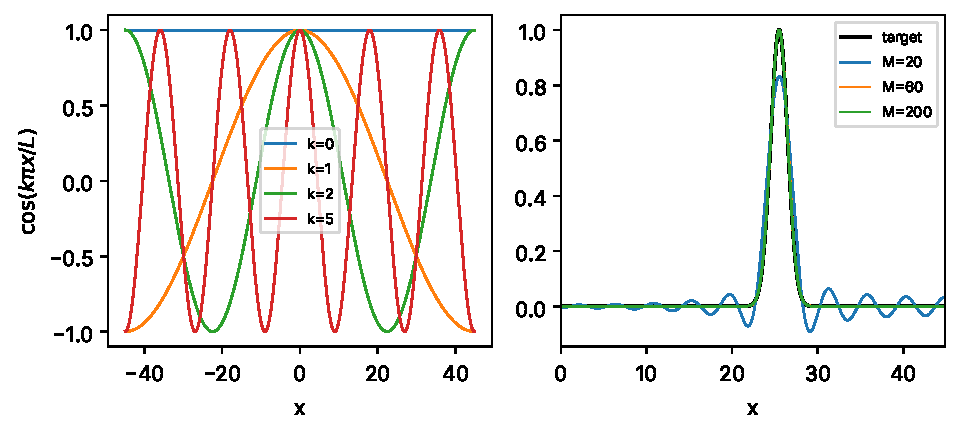
\includegraphics[width=0.95\linewidth]{figs/fourier-series_cosine_basis.pdf}
\caption{Left: cosine basis functions $\cos(k\pi x/L)$ on the paper's scale-1 box, $L=44.883$, for $k=0,1,2,5$. Each is even and has slope zero at $x=0$. Right: an even target made of two narrow bumps centered at $|x|=25.5$ (black) and its truncated cosine series with $M=20$, $60$ and $200$ terms. Building a narrow localized feature requires cosines whose wavelength $2L/k$ is comparable to its width. $x$ is in units with $\hbar=2m=1$.}
\label{fig:fourier-series-cosine-basis}
\end{figure}

\begin{pycode}
import numpy as np
from scipy.integrate import trapezoid

L = 44.883                      # scale-1 half-width (RE3)
x = np.linspace(-L, L, 20001)
f = np.abs(x)                   # an even target
M = 4
c = np.empty(M)
c[0] = trapezoid(f, x)/(2*L)    # paper convention: c_0 is the average
for k in range(1, M):
    c[k] = trapezoid(f*np.cos(k*np.pi*x/L), x)/L
g = sum(c[k]*np.cos(k*np.pi*x/L) for k in range(M))
print(c)                        # approx [22.44, -18.19, 0, -2.02]
print(np.sqrt(trapezoid((f - g)**2, x)/(2*L)))   # approx 0.621
\end{pycode}

\begin{checkpoint}
Is the $2L$-periodic extension of an even function on $[-L,L]$ continuous at $x=\pm L$? Is the extension of the odd function $f(x)=x$?
\end{checkpoint}
\checkanswer{Even: yes, because $f(-L)=f(L)$. Odd $f(x)=x$: no, it jumps from $L$ to $-L$, a jump of $2L$, so its sine series shows Gibbs overshoot at the walls and coefficients falling like $1/k$.}

\begin{keyideas}
\item Even $\times$ even and odd $\times$ odd are even; even $\times$ odd is odd. Odd functions integrate to zero over $[-L,L]$.
\item Even functions have pure cosine series; odd functions have pure sine series.
\item The cosine basis $\cos(k\pi x/L)$ on $[-L,L]$, with $c_0=\frac1{2L}\int f$ and $c_k=\frac1L\int f\cos\frac{k\pi x}{L}$, has no wall discontinuity for even $f$; kinks give $1/k^2$ decay.
\item Heuristic (top-hat example, \cref{eq:fourier-series-tophat}): a feature of width $w$ needs cosines of wavelength down to about $w$, that is $k$ up to order $2L/w$.
\end{keyideas}

%=====================================================================
\section{Quasi-periodic sums: frequencies that never line up}\label{sec:fourier-series-quasi}

Everything so far concerned functions that repeat. Now add two sinusoids whose periods do not fit together, and something genuinely new happens.

\subsection{When is a sum of two sinusoids periodic?}

Two angular frequencies $\omega_1,\omega_2>0$ are called \textbf{commensurate} if their ratio is rational, $\omega_2/\omega_1=l/j$ with positive integers $j,l$, and \textbf{incommensurate} otherwise.

\paragraph{Theorem (proved).} \emph{A two-frequency sum is periodic exactly when the frequencies are commensurate.} Let $f(t)=\sin(\omega_1t)+\sin(\omega_2t)$ with $0<\omega_1<\omega_2$. Then $f$ is periodic if and only if $\omega_2/\omega_1$ is rational (a ratio of two integers; $\mathbb{Q}$ denotes the set of rational numbers).

\textbf{Proof.}

\textbf{Step 1 (rational $\Rightarrow$ periodic).} If $\omega_2/\omega_1=l/j$, set $\tau=2\pi j/\omega_1$. Then $\omega_1\tau=2\pi j$ and $\omega_2\tau=2\pi j\,\omega_2/\omega_1=2\pi l$, whole numbers of turns, so both terms, and hence $f$, satisfy $f(t+\tau)=f(t)$.

\textbf{Step 2 (periodic $\Rightarrow$ rational): set up.} Suppose $f(t+\tau)=f(t)$ for all $t$ with some $\tau>0$. Differentiating this identity twice with respect to $t$ gives $f''(t+\tau)=f''(t)$.

\textbf{Step 3: isolate one frequency.} $f''(t)=-\omega_1^2\sin\omega_1t-\omega_2^2\sin\omega_2t$, so
\[
g(t)\equiv\omega_2^2f(t)+f''(t)=(\omega_2^2-\omega_1^2)\sin\omega_1t .
\]
Since $f$ and $f''$ both have period $\tau$, so does $g$. Because $\omega_2^2-\omega_1^2\neq0$, $\sin(\omega_1(t+\tau))=\sin(\omega_1t)$ for all $t$.

\textbf{Step 4: conclude for $\omega_1$.} Choose $t$ with $\omega_1t=\pi/2$: then $\sin(\pi/2+\omega_1\tau)=1$, which requires $\omega_1\tau=2\pi j$ for a positive integer $j$ (positive because $\tau>0$).

\textbf{Step 5: the other frequency.} The same steps with $\omega_1^2f+f''=(\omega_1^2-\omega_2^2)\sin\omega_2t$ give $\omega_2\tau=2\pi l$.

\textbf{Step 6: divide.} $\omega_2/\omega_1=l/j$, rational.
\[
\boxed{\sin\omega_1t+\sin\omega_2t\ \text{is periodic}\iff\omega_2/\omega_1\in\mathbb{Q}}
\]
This completes the proof. $\square$

\paragraph{Amplitudes and phases.} The proof is unchanged in substance for $f(t)=A_1\sin(\omega_1t+\varphi_1)+A_2\sin(\omega_2t+\varphi_2)$ with $A_1,A_2\neq0$. Step~1: a shift $\tau=2\pi j/\omega_1$ still adds $2\pi j$ and $2\pi l$ to the two phases, whatever $\varphi_1,\varphi_2$ are. Step~3 becomes $\omega_2^2f+f''=(\omega_2^2-\omega_1^2)A_1\sin(\omega_1t+\varphi_1)$; dividing by the nonzero constant $(\omega_2^2-\omega_1^2)A_1$ shows that $\sin(\omega_1t+\varphi_1)$ has period $\tau$. Step~4: choose $t$ with $\omega_1t+\varphi_1=\pi/2$; then $\sin(\pi/2+\omega_1\tau)=1$ forces $\omega_1\tau=2\pi j$ as before. Step~5 swaps the indices.

\paragraph{Many frequencies.} Let $F(t)=\sum_{j=1}^{J}A_j\sin(\omega_jt+\varphi_j)$ with distinct positive frequencies $\omega_j$ and nonzero amplitudes $A_j$, and suppose $F(t+\tau)=F(t)$ for all $t$, with $\tau>0$. For each $j$ define the operation $D_jg=\omega_j^2g+g''$. Differentiating $g(t+\tau)=g(t)$ shows that derivatives of a $\tau$-periodic function are $\tau$-periodic, so $D_j$ turns $\tau$-periodic functions into $\tau$-periodic functions. On a single term, $D_j\sin(\omega_it+\varphi_i)=(\omega_j^2-\omega_i^2)\sin(\omega_it+\varphi_i)$: $D_j$ kills term $j$ and multiplies every other term by a constant. Fix $i$ and apply $D_j$ once for each $j\neq i$. Every term except term $i$ is killed, and what remains is $C_iA_i\sin(\omega_it+\varphi_i)$, where $C_i=\prod_{j\neq i}(\omega_j^2-\omega_i^2)$ (the product of these factors over all $j\neq i$) is nonzero; this remainder is $\tau$-periodic. Exactly as in Step~4, $\omega_i\tau=2\pi l_i$ for a positive integer $l_i$. Hence every ratio $\omega_i/\omega_1=l_i/l_1$ is rational. Equivalently: \emph{if two frequencies of a finite sum of sinusoids (with nonzero amplitudes) have an irrational ratio, the sum is not periodic.}

\subsection{The logarithms of primes are incommensurate}

Is $\log3/\log2$ rational? Suppose $\log3/\log2=a/b$ with positive integers $a,b$. Then $b\log3=a\log2$, so $\log(3^b)=\log(2^a)$, and since $\log$ is one-to-one, $3^b=2^a$. But $2^a$ is even and $3^b$ is odd. Contradiction. Therefore
\begin{equation}
\frac{\log3}{\log2}=1.5849625\ldots\quad\text{is irrational},
\end{equation}
and by the theorem, $\sin(t\log2)+\sin(t\log3)$ is \textbf{not periodic}: it never exactly repeats itself.

The same argument works for powers of two different primes $p\neq q$: $\log p^m/\log q^{m'}=a/b$ would mean $p^{mb}=q^{m'a}$, two different factorizations of one integer into primes. Ruling that out for general primes needs the uniqueness of prime factorization, proved in Chapter~\ref{ch:primes}; for $2$ against an odd prime, the parity argument above is enough. Powers of the \emph{same} prime behave differently: $\log p^m/\log p^{m'}=m/m'$ is rational, so for example $\log4=2\log2$ and $\log8=3\log2$ are commensurate; they are harmonics of $\log p$.

\subsection{It never repeats, but it comes close}

Let $f(t)=\sin(t\log2)+\sin(t\log3)$. Its largest conceivable value is $2$, reached only if both sines equal $1$ at once: $t\log2=\pi/2+2\pi j$ and $t\log3=\pi/2+2\pi l$. Dividing, $\log3/\log2=(1+4l)/(1+4j)$, rational, which is impossible. So \emph{$f$ never equals $2$}. Yet it comes as close as you like.

\begin{sample}{Getting close to the maximum}
Find a $t$ in $[0,200]$ where $f(t)=\sin(t\log2)+\sin(t\log3)$ exceeds $1.999$.

\textbf{Step 1: put the first sine at its peak.} Take $t=(\pi/2+2\pi j)/\log2$; then $\sin(t\log2)=1$.

\textbf{Step 2: phase of the second sine.} Its phase is $t\log3=(\pi/2+2\pi j)\rho$ with $\rho=\log3/\log2=1.58496$. We want this to be close to $\pi/2$ modulo $2\pi$, that is, after discarding whole turns of $2\pi$.

\textbf{Step 3: scan $j$.} We need the second phase within $\arccos(0.999)=0.0447$ rad of $\pi/2$ (modulo $2\pi$), so that the second sine exceeds $0.999$. Computing this mismatch for $j=0,1,2,\dots$ in turn (a short loop, rerun in CHECKS) gives, for example, $0.62$ rad at $j=3$ and $0.45$ rad at $j=5$; the first $j$ with mismatch below $0.0447$ is $j=10$. For $j=10$: $t=20.5\pi/\log 2=92.913$, and $t\log3=102.0759$. Subtracting $16\times2\pi=100.5310$ leaves $1.5449$, which is $0.0259$ below $\pi/2=1.5708$.

\textbf{Step 4: value.} $\sin(1.5449)=\cos(0.0259)=0.99967$, so
\[
\boxed{f(92.913)=1.99967}
\]
\end{sample}

\paragraph{Near-periods.} Similarly, $f$ never satisfies $f(t+\tau)=f(t)$ exactly, but it nearly does for special $\tau$. Take $\tau$ equal to $a$ periods of the $\log2$ term, $\tau=2\pi a/\log2$, so the first sine returns exactly. The second sine has advanced by $\tau\log3/(2\pi)=a\rho$ cycles; if $a\rho$ is close to a whole number, it nearly returns too. Writing $\varepsilon$ for the distance of $a\rho$ from the nearest integer (in cycles), the shift of the second term changes its phase by $\delta=2\pi\varepsilon$ (modulo $2\pi$). To compare $\sin(\beta+\delta)$ with $\sin\beta$, replace $\beta$ by $-\beta$ in \cref{eq:fourier-series-sumprod}, using $\sin(-\beta)=-\sin\beta$ and $\cos(-u)=\cos u$: $\sin\alpha-\sin\beta=2\cos\frac{\alpha+\beta}{2}\sin\frac{\alpha-\beta}{2}$. Now set $\alpha=\beta+\delta$:
\begin{equation}
\sin(\beta+\delta)-\sin\beta=2\cos\!\left(\beta+\tfrac\delta2\right)\sin\tfrac\delta2,
\end{equation}
whose largest absolute value over $\beta$ is $2|\sin(\delta/2)|=2|\sin(\pi\varepsilon)|$. So
\begin{equation}
\max_t|f(t+\tau)-f(t)|=2|\sin(\pi\varepsilon)|\qquad(\tau=2\pi a/\log2).
\label{eq:fourier-series-nearperiod}
\end{equation}
\Cref{tab:fourier-series-nearperiods} lists the best $a$ up to 53. For a general shift $\tau$, not of this special form, we measure the mismatch by $D(\tau)=\sup_t|f(t+\tau)-f(t)|$. Here $\sup$ (the \textbf{supremum}, or least upper bound) is the smallest number that the quantity never exceeds as $t$ varies; unlike a maximum, it need not be attained at any $t$.

\begin{table}[htbp]\centering
\caption{Near-periods of $f(t)=\sin(t\log2)+\sin(t\log3)$ built from $a$ periods of the $\log 2$ term. $\varepsilon$ is the distance of $a\log3/\log2$ from the nearest integer; the last column is \cref{eq:fourier-series-nearperiod}.}
\label{tab:fourier-series-nearperiods}
\begin{tabular}{rrrrr}
\toprule
$a$ & $\tau=2\pi a/\log2$ & $a\log3/\log2$ & $\varepsilon$ & $\max_t|f(t+\tau)-f(t)|$\\
\midrule
1 & 9.065 & 1.58496 & 0.41504 & 1.929\\
2 & 18.129 & 3.16993 & 0.16993 & 1.018\\
5 & 45.324 & 7.92481 & 0.07519 & 0.468\\
12 & 108.777 & 19.01955 & 0.01955 & 0.1228\\
41 & 371.654 & 64.98346 & 0.01654 & 0.1039\\
53 & 480.430 & 84.00301 & 0.00301 & 0.0189\\
\bottomrule
\end{tabular}
\end{table}

The row $a=12$ is a near-coincidence musicians know: $12\log3\approx19\log2$ means $3^{12}\approx2^{19}$ ($531441$ against $524288$, a ratio of $1.01364$ called the Pythagorean comma). That is why twelve equal semitones nearly, but not exactly, produce perfect fifths. The row $a=53$ says $3^{53}\approx2^{84}$, within a factor $1.0021$.

\begin{figure}[htbp]\centering
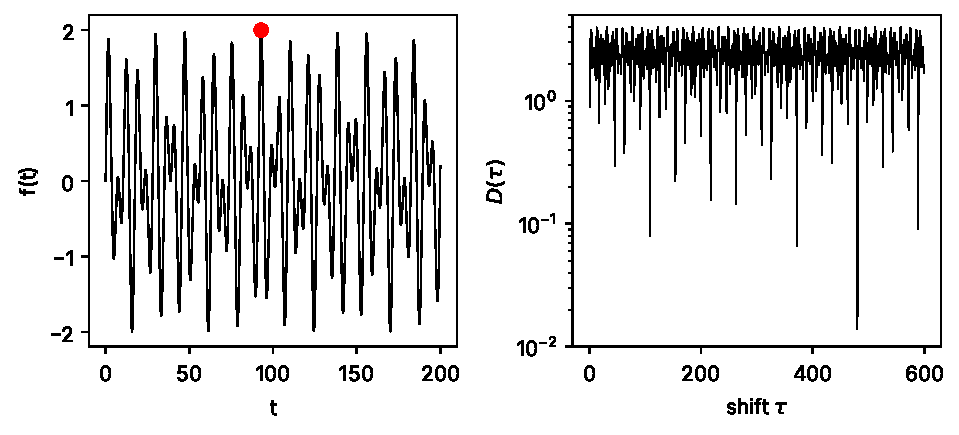
\includegraphics[width=0.95\linewidth]{figs/fourier-series_quasiperiodic.pdf}
\caption{Left: the quasi-periodic sum $f(t)=\sin(t\log2)+\sin(t\log3)$; the dot marks $t=92.913$ where $f=1.99967$, close to (but below) the never-attained value $2$. Right: the largest mismatch $D(\tau)=\sup_t|f(t+\tau)-f(t)|$ as a function of the shift $\tau$ (logarithmic scale). It dips near $\tau=108.8$ and $480.4$ (\cref{tab:fourier-series-nearperiods}) but never reaches zero. All axes dimensionless.}
\label{fig:fourier-series-quasiperiodic}
\end{figure}

\begin{beyond}
\textbf{Kronecker's theorem and almost periodic functions.} Two facts used informally here are proved elsewhere. (1) Kronecker's theorem: if $\omega_1/\omega_2$ is irrational, the pair of phases $(\omega_1t,\omega_2t)$ modulo $2\pi$ comes arbitrarily close to every pair of angles as $t$ ranges over the reals. Consequently $\sup_tf=2$ (approached, never reached), because both phases can be brought, at the same $t$, as close as we like to $\pi/2$. Likewise, for a general shift $\tau$ write $f(t+\tau)-f(t)=[\sin(\alpha+\delta_2)-\sin\alpha]+[\sin(\beta+\delta_3)-\sin\beta]$ with $\alpha=t\log2$, $\beta=t\log3$, $\delta_2=\tau\log2$, $\delta_3=\tau\log3$. By the difference identity used for \cref{eq:fourier-series-nearperiod}, the two brackets have largest absolute values $2|\sin(\delta_2/2)|$ and $2|\sin(\delta_3/2)|$, and Kronecker's theorem lets $\alpha$ and $\beta$ approach, at the same $t$, angles where both brackets are near their maxima with the same sign. So the supremum of the mismatch (approached, in general not attained) is $D(\tau)=2|\sin(\tau\log2/2)|+2|\sin(\tau\log3/2)|$, the formula plotted in \cref{fig:fourier-series-quasiperiodic}. A proof is in Hardy and Wright~\cite{hardywright}, chapter XXIII. (2) H.~Bohr's theory of \emph{almost periodic functions}: a finite sum of sinusoids with any real frequencies has, for every $\epsilon>0$, ``$\epsilon$-almost-periods'' $\tau$ with $|f(t+\tau)-f(t)|<\epsilon$ for all $t$, and such $\tau$ occur with bounded gaps along the whole real line. Functions of this kind are called almost periodic or quasi-periodic. Bohr's theory, including the existence of $\epsilon$-almost-periods with bounded gaps, is developed with proofs in his monograph \emph{Almost Periodic Functions} and in later texts on harmonic analysis. We take both results on trust; we use only the conclusions stated.
\end{beyond}

\subsection{Long-time averages and Parseval for quasi-periodic sums}

Over a period, orthogonality killed cross terms exactly. A quasi-periodic sum has no period, but cross terms still die in the long run. Define the average over a window of length $T$ starting at $0$: $\langle g\rangle_T=\frac1T\int_0^Tg\,\dd t$. For $\omega_1\neq\omega_2$, by \cref{eq:fourier-series-ps},
\begin{align}
\langle\sin\omega_1t\sin\omega_2t\rangle_T&=\frac1{2T}\int_0^T\left[\cos(\omega_1-\omega_2)t-\cos(\omega_1+\omega_2)t\right]\dd t\\
&=\frac1{2T}\left[\frac{\sin(\omega_1-\omega_2)T}{\omega_1-\omega_2}-\frac{\sin(\omega_1+\omega_2)T}{\omega_1+\omega_2}\right],
\end{align}
and since $|\sin|\le1$,
\begin{equation}
\left|\langle\sin\omega_1t\sin\omega_2t\rangle_T\right|\le\frac1{2T}\left(\frac1{|\omega_1-\omega_2|}+\frac1{\omega_1+\omega_2}\right)\xrightarrow{T\to\infty}0 .
\label{eq:fourier-series-avgorth}
\end{equation}
With $\omega_1=\omega_2=\omega$, \cref{eq:fourier-series-ps} gives $\langle\sin^2\omega t\rangle_T=\frac12-\frac{\sin2\omega T}{4\omega T}\to\frac12$. Phase constants change nothing. By \cref{eq:fourier-series-ps}, $\sin(\omega_1t+\varphi_1)\sin(\omega_2t+\varphi_2)=\tfrac12[\cos((\omega_1-\omega_2)t+\varphi_1-\varphi_2)-\cos((\omega_1+\omega_2)t+\varphi_1+\varphi_2)]$, and for $\Omega\neq0$, $\frac1T\int_0^T\cos(\Omega t+\psi)\,\dd t=\frac{\sin(\Omega T+\psi)-\sin\psi}{\Omega T}$, which is at most $2/(|\Omega|T)$ in size. So the cross-term average is bounded by $\frac1T\big(\frac1{|\omega_1-\omega_2|}+\frac1{\omega_1+\omega_2}\big)$ and again tends to zero; and $\sin^2(\omega t+\varphi)=\tfrac12-\tfrac12\cos(2\omega t+2\varphi)$ has average within $1/(2\omega T)$ of $\tfrac12$. Now take a finite sum $F(t)=\sum_jA_j\sin(\omega_jt+\varphi_j)$ with \emph{distinct} frequencies and expand its square: $F^2=\sum_jA_j^2\sin^2(\omega_jt+\varphi_j)+\sum_{i\neq j}A_iA_j\sin(\omega_it+\varphi_i)\sin(\omega_jt+\varphi_j)$. The square terms average to $A_j^2/2$ and the cross terms to zero as $T\to\infty$, so
\begin{equation}
\lim_{T\to\infty}\langle F^2\rangle_T=\sum_j\frac{A_j^2}{2},
\label{eq:fourier-series-parsevalqp}
\end{equation}
Parseval's theorem for quasi-periodic sums. The bound \cref{eq:fourier-series-avgorth} carries a lesson for later: two frequencies only ``look orthogonal'' once $T$ is large compared with $1/|\omega_1-\omega_2|$. Telling close frequencies apart needs a long window. Chapter~\ref{ch:fourier-transform} turns this into the resolution $\Delta\omega\approx2\pi/T$.

\begin{checkpoint}
Is $\sin(t\log4)+\sin(t\log8)$ periodic? If so, find its period.
\end{checkpoint}
\checkanswer{Yes: $\log4=2\log2$ and $\log8=3\log2$, ratio $3/2$. Both are harmonics of $\log2$, so the period is $2\pi/\log2=9.065$.}

\begin{keyideas}
\item $\sin\omega_1t+\sin\omega_2t$ is periodic if and only if $\omega_2/\omega_1$ is rational (proved).
\item $\log3/\log2$ is irrational (parity proof); logarithms of powers of \emph{different primes} are incommensurate (unique factorization, Chapter~\ref{ch:primes}), while powers of the same prime are harmonics of $\log p$.
\item A finite sum of sinusoids with nonzero amplitudes is periodic only if all its frequency ratios are rational (proved, many-frequency version).
\item Quasi-periodic sums never repeat exactly but have near-periods, \cref{tab:fourier-series-nearperiods}.
\item Long-time averages kill cross terms between distinct frequencies, so mean squares still add, \cref{eq:fourier-series-parsevalqp}, once $T\gg1/|\Delta\omega|$.
\end{keyideas}

%=====================================================================
\section{Why a finite window cannot capture an almost-periodic function}\label{sec:fourier-series-window}

Suppose you know a function only on a window $[0,T]$ and you expand it in a Fourier series on that window. What does the series predict outside?

\subsection{A Fourier series on a window predicts its own periodic extension}

On the window $[0,T]$ (length $T$, so ``$2L$'' $=T$), the complex Fourier series is
\begin{equation}
F(t)=\sum_k\hat f_ke^{2\pi ikt/T},\qquad \hat f_k=\frac1T\int_0^Tf(t)e^{-2\pi ikt/T}\dd t .
\label{eq:fourier-series-windowFS}
\end{equation}
(The derivation is that of \cref{eq:fourier-series-complexFS} with the interval $[0,T]$; orthogonality holds on any interval of length equal to the period.) Each term satisfies $e^{2\pi ik(t+T)/T}=e^{2\pi ikt/T}e^{2\pi ik}=e^{2\pi ikt/T}$, so $F(t+T)=F(t)$. Inside the window, $F=f$ (where $f$ is continuous). Outside, $F$ is forced to repeat the window: for $T<t<2T$, $F(t)=F(t-T)=f(t-T)$. So the prediction error on the next window is
\begin{equation}
F(t)-f(t)=f(t-T)-f(t),\qquad T<t<2T.
\label{eq:fourier-series-extensionerror}
\end{equation}
This vanishes for all such $t$ only if $f$ repeats with period $T$ there.

\textbf{Consequence.} If $f$ is quasi-periodic, like $\sin(t\log2)+\sin(t\log3)$, it has no period at all (\cref{sec:fourier-series-quasi}), so \emph{for every window length $T$}, the window's Fourier series mispredicts somewhere outside the window. The size of the error is set by \cref{eq:fourier-series-nearperiod} and \cref{fig:fourier-series-quasiperiodic}: it is small only for special near-periods and is never zero. Choosing $T$ to fit a whole number of $\log2$ periods cannot also fit a whole number of $\log3$ periods, because that would make $\log3/\log2$ rational.

\begin{figure}[htbp]\centering
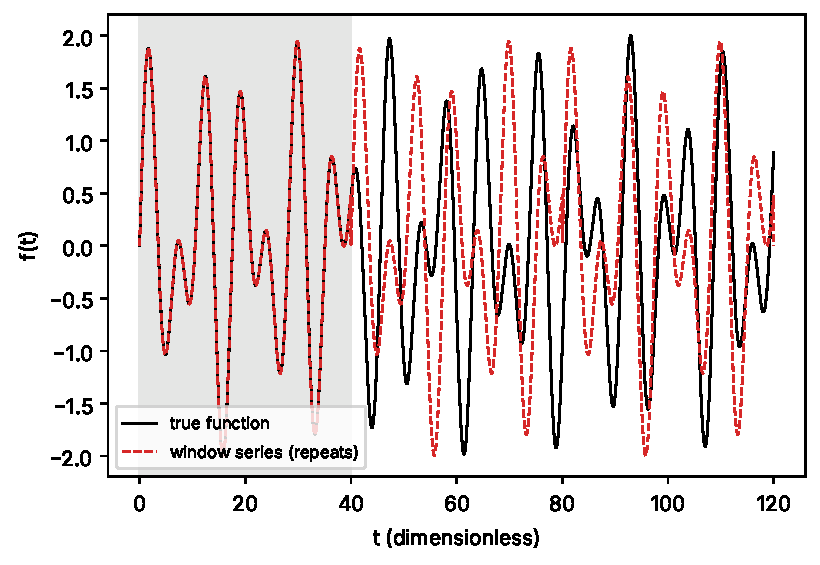
\includegraphics[width=0.85\linewidth]{figs/fourier-series_window.pdf}
\caption{The quasi-periodic function $\sin(t\log2)+\sin(t\log3)$ (solid) and the Fourier series of its window $[0,40]$ (shaded), which inside the window reproduces it and outside merely repeats the window (dashed). The repetition jumps at $t=40$ and $80$ and does not continue the true function. Axes dimensionless.}
\label{fig:fourier-series-window}
\end{figure}

\subsection{Even one sinusoid spreads over many harmonics}

The problem appears even for a single frequency that does not fit the window. Take $f(t)=e^{i\omega t}$ on $[0,T]$ and write $\omega_k=2\pi k/T$ for the window's harmonic frequencies. From \cref{eq:fourier-series-windowFS},
\begin{equation}
\hat f_k=\frac1T\int_0^Te^{i(\omega-\omega_k)t}\dd t=\frac{e^{i(\omega-\omega_k)T}-1}{i(\omega-\omega_k)T}.
\end{equation}
Let $\theta=(\omega-\omega_k)T/2$. Factor $e^{i\theta}$ out of the numerator: $e^{2i\theta}-1=e^{i\theta}(e^{i\theta}-e^{-i\theta})=e^{i\theta}\,2i\sin\theta$. So
\begin{equation}
\hat f_k=e^{i\theta}\,\frac{\sin\theta}{\theta},\qquad |\hat f_k|=\left|\frac{\sin\theta}{\theta}\right|,\qquad \theta=\pi\left(\frac{\omega T}{2\pi}-k\right).
\label{eq:fourier-series-sinc}
\end{equation}
If the window holds a whole number $k_0$ of cycles ($\omega T/2\pi=k_0$), then $\theta=\pi(k_0-k)$, so $\hat f_{k_0}=1$ and every other $\hat f_k=0$: one harmonic. Otherwise \emph{every} $\hat f_k$ is nonzero, falling off only like $1/|k|$, the signature of the jump that the periodic extension creates at the window edge. The function $\sin\theta/\theta$ (the ``sinc'') is the subject of the next chapter.

\begin{sample}{A window that does not fit the prime-2 frequency}
For $f(t)=e^{it\log2}$ on a window of length $T=40$, find the number of cycles in the window and $|\hat f_4|$, $|\hat f_5|$.

\textbf{Step 1: cycles.} $\omega T/2\pi=40\times0.693147/6.283185=4.4127$, not a whole number.

\textbf{Step 2: $k=4$.} $\theta=\pi(4.4127-4)=1.2966$, $|\hat f_4|=\sin(1.2966)/1.2966=0.742$.

\textbf{Step 3: $k=5$.} $\theta=\pi(4.4127-5)=-1.8450$, $|\hat f_5|=\sin(1.8450)/1.8450=0.522$.
\[
\boxed{|\hat f_4|=0.742,\qquad|\hat f_5|=0.522}
\]
A single pure frequency is smeared over the window's harmonics. Choosing $T=2\pi\cdot4/\log 2=36.26$ instead would put exactly four cycles in the window and give a single harmonic.
\end{sample}

\subsection{Representing is not continuing}

Here is the lesson in plain words. A flexible enough set of building blocks can \emph{represent} any function on a window as closely as you like. That says nothing about whether the blocks \emph{continue} the function correctly outside the window. The window Fourier series reproduces the window perfectly and then repeats it, because ``repeat with period $T$'' is the only continuation its vocabulary can express. To continue $\sin(t\log2)$ correctly, a model needs to contain the frequency $\log2$ itself, not an imitation of one window of it. We will meet this distinction again as \emph{memorization versus generalization} (Chapter~\ref{ch:generalization}) and as \emph{sparse frequency learning} (Chapter~\ref{ch:sparse-frequency}).

\begin{keyideas}
\item The Fourier series of a window $[0,T]$ equals the function inside and its $T$-periodic repetition outside, \cref{eq:fourier-series-extensionerror}.
\item A quasi-periodic function is not $T$-periodic for any $T$, so no window's periodic extension continues it correctly.
\item A sinusoid whose frequency does not fit the window spreads over all harmonics with weights $|\sin\theta/\theta|$, \cref{eq:fourier-series-sinc}.
\item Fitting a window (representation) and continuing beyond it (prediction) are different abilities.
\end{keyideas}

%=====================================================================
\section{Paper connection}\label{sec:fourier-series-paper}

\subsection{The cosine basis of \texorpdfstring{$\delta V$}{delta V} (paper Sec.~II~C)}

The Hermitian model of the paper~\cite{soniR1} (Sec.~II~C) perturbs the even Wu--Sprung potential by
\begin{equation}
\delta V(x)=\sum_{k=0}^{M-1}c_k\cos\frac{k\pi x}{L},
\end{equation}
exactly the basis \cref{eq:fourier-series-basis} with the constant convention of \cref{eq:fourier-series-cosconv}. You now know why it is cosines: the background is even (Sec.~II~B, ``with $V$ even''), so an even correction needs no sines (\cref{sec:fourier-series-evenodd}), and the periodic extension of an even function has no jump at the walls $\pm L$. The half-widths are $L=44.883$ at scale~1 and $L=59.957$ at scale~2 (Sec.~II~B), and Table~I uses $M$ from 200 to 900.

What scales can such a basis resolve? The shortest wavelength present is $2L/(M-1)$: for $M=400$ at scale~1 it is $2\times44.883/399=0.225$ (wavenumber $399\pi/L=27.93$); for $M=900$ at scale~2 it is $0.1334$ (Problem~14). The paper's first paragraph of Sec.~III states a basis-coverage law, ``the cosine family becomes effectively complete for joint level shifts once $M\pi/L>2\sqrt E$''. Chapter~\ref{ch:fitting} derives this heuristic; here we only do arithmetic with it. For level 500 at scale~1, with $E\approx t_{500}=811.18$ (App.~A key anchors), it requires $M>2\sqrt{811.18}\times44.883/\pi=813.8$, consistent with the paper's report that $M=900$ reproduces all 500 zeros to rms $<10^{-4}$ spacings. For $M=400$, $M\pi/L=28.0$, so the law covers only levels with $2\sqrt E<28.0$, that is $E$ below about 196.

The interpolation split (Sec.~III, Fig.~4) shows the superposition principle at work: the fitted cosine series builds a localized structure, ``rms $\delta V=40$'' in the band $x=22.5$--$28.5$ ``against 15 inside it and 13 outside it, with a maximum $|\delta V|=199$''. A correction that is largest in a band of width 6 (the classical turning points of the held-out levels 201--300, Chapter~\ref{ch:wkb}) while remaining nonzero elsewhere (rms 15 and 13) is a superposition of many cosines, as in \cref{fig:fourier-series-cosine-basis} and the top-hat example of \cref{sec:fourier-series-evenodd} (for $w=6$ at scale~1 the main lobe extends to $k\approx2L/w=14.96$); the highest $M=400$ cosine fits about 27 wavelengths into that band (Problem~27).

The even/odd rules also explain a detail of Sec.~II~E. The PT-odd class uses the \emph{odd} basis $\sin((k+1)\pi x/L)$ and the paper notes $A_{nn}=0$. In an even potential each $|\psi_n|^2$ is even (Chapter~\ref{ch:bound-states}), so $A_{nn}=\int|\psi_n|^2\,(\text{odd})\,\dd x$ integrates an odd function over $[-L,L]$ and vanishes by \cref{sec:fourier-series-evenodd}. The absorptive-even class uses the cosines, whose $k=0$ member is the constant $\phi_0=1$; its special ``null mode'' role is the subject of Chapter~\ref{ch:non-hermitian}.

\subsection{Paper Eq.~(4) is an almost-periodic sum}

The arithmetic oracle, paper Eq.~(4),
\begin{equation}
\Nfl(t)=-\frac1\pi\sum_{p\in P}\sum_{m=1}^{3}\frac{\sin(mt\log p)}{m\,p^{m/2}},
\end{equation}
is a finite sum of sinusoids in $t$ with amplitudes $1/(\pi mp^{m/2})$ and angular frequencies $m\log p=\log p^m$. (Here $P$ is the paper's set of primes, not a period.) Within one prime the three frequencies are harmonics of $\log p$, so a one-prime oracle is periodic with period $2\pi/\log p$. Across different primes the frequencies are incommensurate (\cref{sec:fourier-series-quasi}); for example $\log3/\log2$ is irrational. With two or more primes, $\Nfl$ is a finite sum of sinusoids with distinct frequencies and nonzero amplitudes, two of which have an irrational ratio, so by the many-frequency version of the periodicity theorem (\cref{sec:fourier-series-quasi}) it is not periodic: it is quasi-periodic and never repeats. The six-prime oracle of Fig.~1 uses the six smallest primes, $P=\{2,3,5,7,11,13\}$ (the paper says only ``six-prime''; this is the natural reading, it is what \texttt{qmnt.first\_primes(6)} returns, and with it \texttt{qmnt} reproduces the six-prime entry $0.074$ / $+0.96$ of Table~V on zeros 401--500), and has $6\times3=18$ distinct frequencies (Problem~26). Chapter~\ref{ch:explicit-formula} explains where Eq.~(4) comes from; this chapter explains what kind of function it is. Because it is a sum of sinusoids with \emph{known} frequencies, it is defined for every $t$, and it continues automatically past any training window; nothing in it needs to be learned from the zeros. That is the property the fitted potentials, as parametrized and optimized in the paper, did not show.

The paper's Discussion (Sec.~VI) puts its heuristic explanation of the failure in exactly these terms: ``the quantity being fitted is, by the explicit formula, an almost-periodic function of $t$ that is sparse in frequency, whereas a potential addresses the levels through their turning points, locally in energy.'' The paper labels this reading heuristic, and so do we.

\subsection{The prime-2 wave in level index}

RE2 is the $p=2$ part of Eq.~(4). Its period in $t$ is $2\pi/\log2=9.065$. The paper scores levels by their index $n$, and consecutive levels near zero $n$ are about one local mean spacing $\gap_n=2\pi/\log(s_n/2\pi)$ apart (Chapter~\ref{ch:counting-zeros}), where $s_n$ is the smooth zero. So one period of RE2 spans $9.065/\gap_n$ levels. Solving $\Nsm(s_n)=n-\tfrac12$ numerically gives $s_{400}=679.9$, $\gap_{400}=1.341$ and $9.065/1.341=6.76$ levels per period; at $n=500$, $\gap_{500}=1.293$ and $7.01$ levels per period. So one period is about 7 levels, in line with the paper's approximate remark in Sec.~V that the $p=2$ oscillation ``is only $\sim$6--7 \emph{levels} at these heights''; our value $7.01$ at $n=500$ sits at the upper edge of that rounded range. \Cref{fig:fourier-series-re2-levels} shows RE2 sampled at the smooth zeros: perfectly periodic in $t$, it looks only roughly regular in $n$, because the mean spacing shrinks slowly with height.

\begin{figure}[htbp]\centering
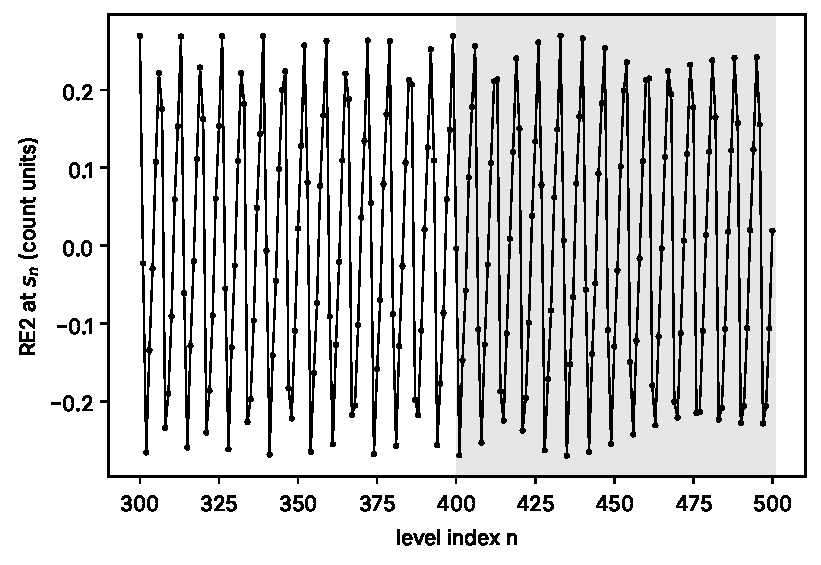
\includegraphics[width=0.85\linewidth]{figs/fourier-series_re2_levels.pdf}
\caption{The prime-2 wave RE2 (the $p=2$, $m\le3$ part of paper Eq.~(4)) evaluated at the smooth zeros $s_n$, $n=300$--$500$. One period ($9.065$ in $t$) spans about 6.4 levels at $n=300$ and 7.0 at $n=500$. The shaded region $n=401$--$500$ is the held-out window of the paper's continuation probe (Sec.~III), whose target is the negative of this sequence (App.~A step 15). Vertical axis: count units, equivalently mean spacings.}
\label{fig:fourier-series-re2-levels}
\end{figure}

\begin{pycode}
import numpy as np
from scipy.optimize import brentq

def Nsm(t):                        # paper Eq. (1)
    return t/(2*np.pi)*np.log(t/(2*np.pi)) - t/(2*np.pi) + 7/8

def smooth_zero(n):                # s_n: Nsm(s_n) = n - 1/2
    return brentq(lambda t: Nsm(t) - (n - 0.5), 2*np.pi, 1e5)

def re2(t):                        # RE2: the p = 2 part of Eq. (4)
    m = np.arange(1, 4)
    return -np.sum(np.sin(np.outer(t, m*np.log(2)))/(m*2**(m/2)), axis=1)/np.pi

for n in (400, 500):
    s = smooth_zero(n)
    gap = 2*np.pi/np.log(s/(2*np.pi))
    print(n, s, gap, (2*np.pi/np.log(2))/gap)    # levels per period

s = np.array([smooth_zero(n) for n in range(401, 501)])
print("rms of RE2 on 401-500:", np.sqrt(np.mean(re2(s)**2)))
\end{pycode}

\subsection{The arithmetic-continuation probe (paper Sec.~III, App.~A step 15)}

The probe replaces the true targets by the synthetic fluctuation $-N^{p=2}_{\rm fl}(s_n)$ in mean spacings (App.~A step 15 defines targets $T_n=E_n[\text{smooth}]-N^{p=2}_{\rm fl}(s_n)\,\gap_n$; this $T_n$ is a target level, not a window length). In other words, the target fluctuation is $-$RE2 sampled at the smooth zeros, the negative of the sequence in \cref{fig:fourier-series-re2-levels}: a target level sits below its smooth position when the count fluctuation is positive. The sign affects neither the rms nor the period. The fitted potential is trained on levels 1--400 and asked to continue on 401--500.

Parseval tells us what ``doing nothing'' costs. The long-run rms of RE2 is $0.1709$ (Sample Problem ``The rms of the prime-2 wave''). The paper's probe null, the rms of predicting zero fluctuation on 401--500, is $0.1708$ (App.~A key anchors). The two agree closely, as they should: levels 401--500 span about 130 in $t$, roughly 14 periods, enough for the cross terms in \cref{eq:fourier-series-avgorth} to be small. (CHECKS recomputes the sample rms on 401--500 and confirms it lies within $0.003$ of both.)

The results (Sec.~III): in-sample rms $0.056$ and correlation $+0.95$; held-out correlation $+0.07$ and held-out rms $0.1958$, worse than the null $0.1708$ (App.~A key anchors). In the paper's words, ``The family can paint one window of $\sin(t\log 2)$ onto its levels but cannot express `continue oscillating': the arithmetic frequency is not in its vocabulary.'' \Cref{sec:fourier-series-window} gives you a precise model of the phrase ``not in its vocabulary'': a window Fourier series also paints its window perfectly and then continues it wrongly, because its only built-in continuation is periodic repetition. This is an analogy, not the paper's mechanism: the potential's cosines live in $x$, not in $t$, and the paper describes its own explanation as heuristic. What the analogy captures is that representing a window and continuing a frequency are different abilities. Notice also that RE2 is exactly periodic in $t$; the probe shows that the failure does not need quasi-periodicity, since ``a single known arithmetic frequency, learned from a finite window, already defeats the family's extrapolation'' (Sec.~III).

\subsection{A Fourier-series view of the dense control C1}

The control C1 (Sec.~II~D, Table~IV, App.~A step 20) fits $F(t)=\sum_j[a_j\sin\omega_jt+b_j\cos\omega_jt]$ on the uniform grid $\omega_j=8j/450$, 450 frequencies and 900 coefficients. Every $\omega_j$ is a whole multiple of $8/450$, so by the argument of \cref{sec:fourier-series-sinusoids} the model is \emph{exactly periodic} with period $2\pi\times450/8=353.43$ in $t$: it is a truncated Fourier series in disguise. Its training zeros run from $t_1=14.13$ up to about $t_{400}\approx680$, and the held-out levels 401--500 sit at heights from about $681$ to $811$, so the model's values there are copies of its values at heights about $328$ to $458$, inside the training range (Problem~15). This is our observation about the form of the model, not a result reported in the paper; the paper reports only that C1 ``stays within $0.005$ of the null'' (rms $0.258$, correlation $+0.28$ with interval $[+0.08,+0.46]$) and concludes that ``capacity without a suitable prior does not generalize''. It illustrates \cref{sec:fourier-series-window} in a model the paper actually ran: a generic periodic vocabulary, however large, continues by repetition.

By contrast, C2 (Sec.~II~D, Sec.~IV) searches for a few frequencies one at a time and finds them at $\log p^m$; that is the subject of Chapter~\ref{ch:sparse-frequency}, built on the periodogram of Chapter~\ref{ch:fourier-transform}.

%=====================================================================
\section{Summary}\label{sec:fourier-series-summary}
% DYK-BEGIN
\begin{didyouknow}{The Overshoot That Won't Quit}
Approximate a square wave by a finite Fourier series and you always see an overshoot near each jump, about 9\% of the jump size, however many terms you keep. It is called the Gibbs phenomenon after J. Willard Gibbs, who discussed it in \emph{Nature} in 1899, but Henry Wilbraham had described it in 1848. Albert Michelson's mechanical harmonic analyzer helped bring it to attention.
\end{didyouknow}
% DYK-END

\begin{itemize}
\item A sinusoid $A\cos(\omega t+\varphi)=a\cos\omega t+b\sin\omega t=\Re[Ze^{i\omega t}]$ has period $2\pi/\omega$, \cref{eq:fourier-series-sinusoid,eq:fourier-series-period,eq:fourier-series-ab,eq:fourier-series-phasor}. RE2 is a sum of three harmonics of $\log2$ with period $2\pi/\log2=9.065$.
\item Two sinusoids of nearby frequencies beat with period $2\pi/\Delta\omega$, \cref{eq:fourier-series-beats,eq:fourier-series-beatperiod}.
\item Sines and cosines of whole-number frequencies on $[-L,L]$ are orthogonal (\cref{tab:fourier-series-orth}); so are complex exponentials, \cref{eq:fourier-series-orthexp}.
\item Fourier series and coefficients: \cref{eq:fourier-series-FS,eq:fourier-series-an,eq:fourier-series-bn}; complex form \cref{eq:fourier-series-complexFS,eq:fourier-series-realcomplex}. Convergence (Dirichlet) is taken on trust.
\item Gibbs: the overshoot of partial sums at a jump tends to about $9\%$ of the jump as the number of terms grows, never to zero, \cref{eq:fourier-series-gibbs}.
\item Parseval: mean squares of orthogonal pieces add, \cref{eq:fourier-series-parseval,eq:fourier-series-parsevalreal}. The rms of RE2 is $0.1709$. Truncated Fourier series are the best mean-square approximations, \cref{eq:fourier-series-best}.
\item Even functions have pure cosine series. The paper's basis is $\cos(k\pi x/L)$ on $[-L,L]$ with $c_0$ equal to the average, \cref{eq:fourier-series-cosconv,eq:fourier-series-basis}. Kinks give $1/k^2$ decay of the coefficients, \cref{eq:fourier-series-decay}; jumps give $1/k$.
\item A two-frequency sum is periodic if and only if the frequency ratio is rational (proved). $\log3/\log2$ is irrational, so sums over several primes, like paper Eq.~(4), are quasi-periodic: they have near-periods (\cref{tab:fourier-series-nearperiods}, \cref{eq:fourier-series-nearperiod}) but no period.
\item Long-time averages give Parseval for quasi-periodic sums, \cref{eq:fourier-series-avgorth,eq:fourier-series-parsevalqp}; separating frequencies needs $T\gg1/|\Delta\omega|$.
\item A window Fourier series continues its window only by repetition, \cref{eq:fourier-series-extensionerror}; an off-grid frequency spreads as $|\sin\theta/\theta|$, \cref{eq:fourier-series-sinc}. Representation is not continuation: the lesson of the paper's continuation probe (Sec.~III).
\end{itemize}

%=====================================================================
\section{Problems}\label{sec:fourier-series-problems}

\begin{problemlist}
\prob{1}{Find the angular frequency and the period of $\sin(t\log3)$, the $p=3$, $m=1$ term of paper Eq.~(4).}

\prob{1}{Write $5\cos\omega t+12\sin\omega t$ in the form $A\cos(\omega t+\varphi)$.}

\prob{1}{The terms $\sin(t\log5)$ and $\sin(t\log7)$ are added with equal amplitudes. Find the beat period.}

\prob{1}{Evaluate $\int_{-L}^{L}\cos^2(5\pi x/L)\,\dd x$ for the scale-2 half-width $L=59.957$, using \cref{tab:fourier-series-orth}.}

\prob{1}{Classify as even, odd or neither: $x^3$, $x\cos x$, $|x|\sin x$, $x\sin x$, $e^x$. For which of them is $\int_{-L}^{L}f\,\dd x=0$ guaranteed?}

\prob{2}{Use complex amplitudes to write $2\cos\omega t+2\cos(\omega t+\pi/3)$ as a single sinusoid.}

\prob{2}{Find the Fourier series of the sawtooth $f(x)=x$ on $(-\pi,\pi)$, extended with period $2\pi$.}

\prob{2}{Apply Parseval's theorem \cref{eq:fourier-series-parsevalreal} to the sawtooth of Problem~7 to obtain $\sum_{k\ge1}1/k^2$.}

\prob{2}{Apply Parseval's theorem to the cosine series of $|x|$ (Sample Problem on $|x|$) to evaluate $\sum_{k\ \rm odd}1/k^4$.}

\prob{2}{Show that over a window of length $T$ that is not a whole number of periods, $\langle\cos^2\omega t\rangle_T=\tfrac12+\sin(2\omega T)/(4\omega T)$. Evaluate it for $\omega=\log2$, $T=10$.}

\prob{2}{What fraction of the mean square of RE2 comes from its $m=1$ term?}

\prob{2}{Verify the Pythagorean comma: compute $3^{12}/2^{19}$ and relate it to the row $a=12$ of \cref{tab:fourier-series-nearperiods}.}

\prob{2}{Prove that $\log5/\log3$ is irrational without using unique factorization in general.}

\prob{2}{(Paper.) Find the shortest wavelength $2L/(M-1)$ in the cosine basis for $M=900$ at scale~2 ($L=59.957$).}

\prob{2}{(Paper.) Show that the dense control C1 (Sec.~II~D, App.~A step 20), with frequencies $\omega_j=8j/450$, is exactly periodic. Find the period and the training heights whose values it reuses on held-out zeros 401--500.}

\prob{2}{(Paper.) Using the coverage law of Sec.~III and $E\approx t_{1000}=1419.42$ (Sec.~II~A), what $M$ would be needed to cover level 1000 at scale~2? Compare with the largest $M$ in Table~I.}

\prob{2}{(Computational.) Using numpy, compute the complex Fourier coefficients $\hat f_k$, $k=-4,\dots,4$, of RE2 over one period $2\pi/\log2$ by numerical integration, and compare with the Sample Problem ``RE2 in complex form''.}

\prob{2}{(Computational, paper.) Using \texttt{qmnt.mean\_gap}, find how many levels one period of the $p=3$ wave $\sin(t\log3)$ spans near $n=400$.}

\prob{3}{(Paper.) Use \cref{eq:fourier-series-parsevalqp} to find the long-time rms of the six-prime oracle $\Nfl$ (paper Eq.~(4) with $P=\{2,3,5,7,11,13\}$). Why can you add the mean squares of all 18 terms?}

\prob{3}{(Computational.) Using numpy, evaluate the Gibbs peak $S_K(\pi/2K)$ for $K=5,10,50,500$ and show that it approaches $1.17898$.}

\prob{2}{Find the mean-square error of approximating the square wave by its first term $(4/\pi)\sin x$.}

\prob{2}{Show that the cosine series of a constant function $f=V_0$ on $[-L,L]$ has $c_0=V_0$ and all other $c_k=0$.}

\prob{2}{Evaluate the near-period entry for $a=5$ in \cref{tab:fourier-series-nearperiods} from \cref{eq:fourier-series-nearperiod}.}

\prob{2}{(Paper.) Using the parity rules, show that $A_{nn}=\int|\psi_n|^2\sin((k+1)\pi x/L)\,\dd x=0$ whenever $|\psi_n|^2$ is even, as stated for the PT-odd class in paper Sec.~II~E.}

\prob{2}{Show by one integration by parts that a function with a jump has Fourier coefficients falling like $1/k$. Use $f(x)=x$ on $(-L,L)$ (odd, jump $2L$ at the walls) as the example.}

\prob{1}{(Paper.) How many distinct frequencies does the six-prime oracle of paper Fig.~1 contain, and what is the largest?}

\prob{1}{(Paper.) How many wavelengths of the highest $M=400$ cosine ($k=399$, scale~1) fit into the band $x=22.5$--$28.5$ of paper Fig.~4?}

\prob{2}{(Computational, paper.) Using \texttt{qmnt.smooth\_zeros} and \texttt{qmnt.mean\_gap}, compute the rms of RE2 sampled at $s_n$ for $n=401$--$500$ and compare with the probe null $0.1708$ (paper App.~A key anchors).}

\prob{3}{Take $f(t)=e^{i\omega t}$ on a window $[0,T]$ holding $k_0+\tfrac12$ cycles. Find $|\hat f_{k_0}|$ and $|\hat f_{k_0+1}|$, and explain why $\sum_k|\hat f_k|^2=1$.}

\prob{3}{(Computational.) Using numpy, build the window Fourier series of $\sin(t\log2)+\sin(t\log3)$ on $[0,40]$ with harmonics $|k|\le40$, and compute its rms error on $[0,40]$ and on $[40,80]$. Interpret with \cref{eq:fourier-series-extensionerror}.}

\prob{2}{Show that RE2 has zero average over a period, and that therefore its $c_0$-type constant term vanishes.}

\prob{3}{(Paper.) Explain, using \cref{sec:fourier-series-window}, why a model that is periodic in $t$ with period shorter than the full data range can never continue paper Eq.~(4) with two or more primes exactly, however many coefficients it has.}
\end{problemlist}

%=====================================================================
\section{Answers to selected problems}\label{sec:fourier-series-answers}

\textbf{1.} $\omega=\log3=1.0986$; $\tau=2\pi/\log3=5.719$.

\textbf{2.} $a=5$, $b=12$, $A=\sqrt{169}=13$; $\cos\varphi=5/13$, $\sin\varphi=-12/13$, so $\varphi=-\arctan(12/5)=-1.176$ rad: $13\cos(\omega t-1.176)$.

\textbf{3.} $\Delta\omega=\log7-\log5=\log1.4=0.33647$; $\tau_{\rm beat}=2\pi/\Delta\omega=18.674$.

\textbf{4.} The $j=k=5\ge1$ case of \cref{tab:fourier-series-orth}: the integral is $L=59.957$.

\textbf{5.} $x^3$ odd; $x\cos x$ odd (odd times even); $|x|\sin x$ odd; $x\sin x$ even (odd times odd); $e^x$ neither ($e^{-x}\neq\pm e^x$). The three odd ones integrate to zero over $[-L,L]$.

\textbf{7.} $f$ is odd, so $a_n=0$. $b_n=\frac2\pi\int_0^\pi x\sin nx\,\dd x$. By parts, $\int_0^\pi x\sin nx\,\dd x=[-x\cos nx/n]_0^\pi+\int_0^\pi\cos nx/n\,\dd x=-\pi(-1)^n/n+0$. So $b_n=2(-1)^{n+1}/n$ and $x=2(\sin x-\tfrac12\sin2x+\tfrac13\sin3x-\cdots)$.

\textbf{9.} Mean square of $|x|$ is $L^2/3$; Parseval gives $L^2/3=c_0^2+\tfrac12\sum c_k^2=L^2/4+\tfrac12\sum_{\rm odd}16L^2/(k^4\pi^4)$. So $1/12=(8/\pi^4)\sum_{\rm odd}k^{-4}$ and $\sum_{\rm odd}1/k^4=\pi^4/96=1.01468$.

\textbf{11.} Mean squares are proportional to $1/(m^22^m)$: $\tfrac12$, $\tfrac1{16}$, $\tfrac1{72}$, total $0.576389$. The $m=1$ fraction is $0.5/0.576389=0.8675$, about $87\%$.

\textbf{13.} If $\log5/\log3=a/b$ with positive integers, then $5^b=3^a$. The right side is divisible by $3$; the left is not, because $5\equiv2$ and powers of $5$ leave remainders $2,1,2,1,\dots$ on division by $3$, never $0$. Contradiction.

\textbf{15.} Every $\omega_j$ is an integer multiple of $8/450$, so by the harmonic argument of \cref{sec:fourier-series-sinusoids} $F(t+\tau)=F(t)$ with $\tau=2\pi\cdot450/8=353.43$. The held-out heights $t_{401}\approx681$ to $t_{500}=811.18$ map to $t-\tau\approx328$ to $457.8$, inside the training range $14.1$--$680$. (Our observation about the model form, not a claim of the paper.)

\textbf{17.} The numerical integrals give $\hat f_{\pm1}=\pm0.1125i$, $\hat f_{\pm2}=\pm0.0398i$, $\hat f_{\pm3}=\pm0.0188i$, and $\hat f_0=\hat f_{\pm4}=0$ to rounding: the window is exactly one period, so there is no leakage.

\textbf{19.} The 18 frequencies $m\log p$ are distinct (different prime powers, Chapter~\ref{ch:primes}), so by \cref{eq:fourier-series-avgorth} every cross term averages to zero and \cref{eq:fourier-series-parsevalqp} applies with $A=1/(\pi mp^{m/2})$: $\langle\Nfl^2\rangle=\frac1{2\pi^2}\sum_p\sum_{m\le3}\frac1{m^2p^m}=\frac{1.472299}{2\pi^2}=0.074588$, rms $0.2731$. (This is a long-run average in $t$ of the oracle function itself, in count units.)

\textbf{21.} By \cref{eq:fourier-series-best} for sines, $\mathcal{E}=\langle f^2\rangle-\tfrac12b_1^2=1-\tfrac12(16/\pi^2)=1-8/\pi^2=0.1894$.

\textbf{23.} $5\log3/\log2=7.92481$, nearest integer $8$, $\varepsilon=0.07519$; $2\sin(\pi\times0.07519)=2\sin(0.23621)=0.468$.

\textbf{25.} For odd $f$, $b_k=\frac2L\int_0^Lf\sin qx\,\dd x$ with $q=k\pi/L$; by parts this is $\frac2L[-f\cos qx/q]_0^L+\frac{2}{Lq}\int_0^Lf'\cos qx\,\dd x$. The boundary term is $-2f(L)(-1)^k/(k\pi)$, which does not shrink faster than $1/k$ unless $f(L)=0$ (no jump). For $f=x$: $f(L)=L$, $f'=1$, the integral term vanishes and $b_k=2L(-1)^{k+1}/(k\pi)$, falling like $1/k$.

\textbf{26.} $6$ primes $\times$ $3$ values of $m$ $=18$ distinct frequencies (distinct prime powers have distinct logarithms). The largest is $3\log13=\log2197=7.695$.

\textbf{27.} Wavelength $2L/399=0.2250$; $6/0.2250=26.7$, about 27 wavelengths.

\textbf{29.} $\theta=\pi(k_0+\tfrac12-k)=\pm\pi/2$ for $k=k_0,k_0+1$, so $|\hat f|=|\sin(\pi/2)/(\pi/2)|=2/\pi=0.6366$ for both. Parseval \cref{eq:fourier-series-parseval} on the window: $\langle|e^{i\omega t}|^2\rangle=1=\sum_k|\hat f_k|^2$, so the weight leaked to all other harmonics is $1-2(4/\pi^2)=0.189$.

\textbf{31.} Each term $\sin(mt\log2)$ integrates to zero over the period $2\pi/\log2$, which contains exactly $m$ of its periods ($I_s$ in \cref{sec:fourier-series-orthogonality}). So the average, which is the constant coefficient, is zero.
